\section{Constrained Dynamics}

Sometimes we are interested in more than simply the number of degrees of freedom a particular configuration has. To explore the configuration space, find similarities between different configurations, analyze the geometric configuration space's topology, or compute other relevant statistics, it can be useful to compute dynamic processes on the constraint space. There are clear computational challenges to computing such dynamics due to computational handling of constraints, the lack of an explicit parameterizations, and the fact that geometric configuration space is often of much smaller dimension than the ambient space it sits in.

Constraint algorithms have been widely studied for use in molecular dynamic simulations. Many  methods use a two stage scheme in which the unconstrained dynamics are first used to evolve the system to an intermediary configuration $\hat{z}_{n+1}$ based on the previous configuration $z_n$. In the second stage, Lagrange multipliers are used to correct $\hat{z}_{n+1}$ to a new configuration $z_{n+1}$ which satisfies the constraints. Previously, we used the SHAKE algorithm--which employs this two stage philosophy--to examine a constraint space used to model the configurations of cyclohexane~\cite{Pandey2014}. 

Assuming connectedness of the configuration space, constraint algorithms can be used to compute various statistics of the configuration space. For example, the $d$-dimensional volume of a $d$-dimensional configuration space can be used to measure how much mobility the intermediate has in its configuration space. Additionally, if we have soft constraints, such as preferred angles between faces, we can institute cost functions on the configuration space with configurations having more favorable angles having a lower cost. Whether physically or artificially motivated, such cost functions can be treated as potential energy functions which can imply specific dynamics. Under this set of dynamics, quantities such as the average or minimum energies may be of interest. 

We may also be interested in the behavior of a small part of the configuration as it undergoes constrained dynamics. For instance, suppose we are interested in the tendency for two edges on distinct faces to come together and form a new connection. By looking at the distance between these edges, we can measure how frequently this event happens and the probability that it will occur before another event of interest. This is similar to the exit time problem for diffusion and may provide a physically motivated evaluation tool for the appropriateness of our transition rules we adopt in our models. 


%\subsection{Cyclohexane Application}

%??include??

%\label{introduction}
%Cyclohexane is a molecule composed of six carbon atoms and twelve hydrogen atoms. The carbon atoms are connected in a ring with two hydrogen atoms attaching to each carbon. Since each carbon has four bonds, the energetically preferred bond spacing is at tetrahedral angles. While this preference dictates much of the cyclohexane structure, there are several structurally distinct conformations the molecule can take. 
%
%Of the many forces acting on the cyclohexane molecule, we focus on three. \textbf{Eclipsing strain} refers to the force between the carbon atoms that prevents them from getting too close to each other. This imposes a preferred distance between each pair of bonded atoms. Second, \textbf{angle strain} corresponds to the carbon atom's four bonds trying to spread apart from each other. As mentioned before, tetrahedral angles are preferred. Finally, \textbf{steric crowding} is similar to eclipsing strain, but the eclipsing in this case is between the hydrogen atoms bonded to the carbons.
%
%\subsubsection{Configurations}
%
%Due to the aforementioned forces, there are a variety of frequently observed configurations with geometries that alleviate these strains to varying amounts. 
%
%The lowest energy configuration is the \textbf{chair}. With the absence of both angle and eclipsing strain, the chair only has a small amount of steric strain. 
%
%Another well studied configuration is the \textbf{boat}. With two sets of parallel carbons arranged in a planar rectangular structure, the remaining two carbon atoms sit at opposite ends slightly above the plain. The structure resembles the bow and stern of a boat. Despite having little angle strain, it does have some steric crowding between the hydrogen atoms at the ends of the boat as well as some eclipsing stain.
%
%
%
%\begin{figure}
%        %\centering
%%        \begin{subfigure}[b]{0.24\textwidth}
%%                \includegraphics[width=\textwidth]{pv_chair_1.png}
%%                %\caption{Chair}
%%                %\label{fig:Chair}
%%        \end{subfigure}%
%%        ~ %add desired spacing between images, e. g. ~, \quad, \qquad etc.
%%          %(or a blank line to force the subfigure onto a new line)
%%        \begin{subfigure}[b]{0.24\textwidth}
%%                \includegraphics[width=\textwidth]{pv_boat_1.png}
%%                %\caption{Boat}
%%                %\label{fig:Boat}
%%        \end{subfigure}%
%%        ~ %add desired spacing between images, e. g. ~, \quad, \qquad etc.
%%          %(or a blank line to force the subfigure onto a new line)
%%        \begin{subfigure}[b]{0.24\textwidth}
%%                \includegraphics[width=\textwidth]{pv_twist_boat_2.png}
%%                %\caption{Twist Boat}
%%                %\label{fig:TwistBoat}
%%        \end{subfigure}%
%%        ~ %add desired spacing between images, e. g. ~, \quad, \qquad etc.
%%          %(or a blank line to force the subfigure onto a new line)
%%        \begin{subfigure}[b]{0.24\textwidth}
%%                \includegraphics[width=\textwidth]{pv_twist_chair_2.png}
%%                %\caption{Twist Chair}
%%                %\label{fig:TwistChair}
%%        \end{subfigure}%
%%
%%        \begin{subfigure}[b]{0.24\textwidth}
%%                \includegraphics[width=\textwidth]{pv_chair_2.png}
%%                %\caption{Chair}
%%                %\label{fig:Chair}
%%        \end{subfigure}%
%%        ~ %add desired spacing between images, e. g. ~, \quad, \qquad etc.
%%          %(or a blank line to force the subfigure onto a new line)
%%        \begin{subfigure}[b]{0.24\textwidth}
%%                \includegraphics[width=\textwidth]{pv_boat_2.png}
%%                %\caption{Boat}
%%                %\label{fig:Boat}
%%        \end{subfigure}%
%%        ~ %add desired spacing between images, e. g. ~, \quad, \qquad etc.
%%          %(or a blank line to force the subfigure onto a new line)
%%        \begin{subfigure}[b]{0.24\textwidth}
%%                \includegraphics[width=\textwidth]{pv_twist_boat_1.png}
%%                %\caption{Twist Boat}
%%                %\label{fig:TwistBoat}
%%        \end{subfigure}%
%%        ~ %add desired spacing between images, e. g. ~, \quad, \qquad etc.
%%          %(or a blank line to force the subfigure onto a new line)
%%        \begin{subfigure}[b]{0.24\textwidth}
%%                \includegraphics[width=\textwidth]{pv_twist_chair_1.png}
%%                %\caption{Twist Chair}
%%                %\label{fig:TwistChair}
%%        \end{subfigure}%
%%
%%        \begin{subfigure}[b]{0.24\textwidth}
%%                \includegraphics[width=\textwidth]{pv_chair_3.png}
%%                \caption{Chair}
%%                \label{fig:Chair}
%%        \end{subfigure}%
%%        ~ %add desired spacing between images, e. g. ~, \quad, \qquad etc.
%%          %(or a blank line to force the subfigure onto a new line)
%%        \begin{subfigure}[b]{0.24\textwidth}
%%                \includegraphics[width=\textwidth]{pv_boat_3.png}
%%                \caption{Boat}
%%                \label{fig:Boat}
%%        \end{subfigure}%
%%        ~ %add desired spacing between images, e. g. ~, \quad, \qquad etc.
%%          %(or a blank line to force the subfigure onto a new line)
%%        \begin{subfigure}[b]{0.24\textwidth}
%%                \includegraphics[width=\textwidth]{pv_twist_boat_3.png}
%%                \caption{Twist Boat}
%%                \label{fig:TwistBoat}
%%        \end{subfigure}%
%%        ~ %add desired spacing between images, e. g. ~, \quad, \qquad etc.
%%          %(or a blank line to force the subfigure onto a new line)
%%        \begin{subfigure}[b]{0.24\textwidth}
%%                \includegraphics[width=\textwidth]{pv_twist_chair_3.png}
%%                \caption{Twist Chair}
%%                \label{fig:TwistChair}
%%        \end{subfigure}%
%%
%%
%%        \caption{Cyclohexane Configurations}\label{fig:animals}
%\end{figure}
%
%
%Besides the chair and boat, there are a few intermediate configurations that cyclohexane assumes as when it transitions between the chair and boat. The aptly named \textbf{twist boat} is similar to the boat, but some of the carbons are rotated from the rest of the molecule. Due to this twisting, the twist boat actually has a lower energy than the boat as the hydrogen atoms at the bow and stern are no longer aligned. Interestingly, the boat can transition via the twist boat to a second boat configuration in which the bow and stern atoms are different, but with an otherwise indistinguishable geometry. As part of the boat's transition to the chair, the \textbf{twist chair} is another distinguished configuration. Having large angle and eclipsing strains, the twist boat represents somewhat of an energy barrier between the chair and boat.  
%
%
%\subsubsection{Finding Intermediate Coordinates}
%
%Since any configuration has an infinitude of equivalent configurations given by rotations and translations, we fix the first three atoms $v_1, v_2,v_3$, at positions $c_1, c_2, c_3$ that satisfy the length and angle constraints. These account for nine of the twenty-one total constraint equations. 
%
%We wish to examine each of the four cyclohexane configurations to verify if they satisfy these constraints, but to do so, an explicit representation of the coordinates of each configuration is required. Since we know from Sachse's model that the boat and chair have a special polyhedral representation, geometry enables us to find such coordinates. We pick the $c_1 = \left(-\sqrt{\frac{2}{3}},0,\sqrt{\frac{1}{3}}\right)$, $c_2 = \left(0,0,0\right)$, $c_3  = \left(\sqrt{\frac{2}{3}},0,\sqrt{\frac{1}{3}}\right)$, and solve for the following coordinates.
%
%\begin{align*}
%v_1^{(chair)} &= \left(-\sqrt{\frac{2}{3}},0,\sqrt{\frac{1}{3}}\right) &= v_1^{(boat)} &= \left(-\sqrt{\frac{2}{3}},0,\sqrt{\frac{1}{3}}\right) \\
%v_2^{(chair)}  &= \left(0,0,0\right) &= v_2^{(boat)}  &= \left(0,0,0\right) \\
%v_3^{(chair)}  &= \left(\sqrt{\frac{2}{3}},0,\sqrt{\frac{1}{3}}\right) &= v_3^{(boat)}  &= \left(\sqrt{\frac{2}{3}},0,\sqrt{\frac{1}{3}}\right) \\
%v_4^{(chair)}  &= \left(\sqrt{\frac{2}{3}},\sqrt{\frac{2}{3}},2\sqrt{\frac{1}{3}}\right) &= v_4^{(boat)}  &= \left(\sqrt{\frac{2}{3}},\sqrt{\frac{2}{3}},2\sqrt{\frac{1}{3}}\right) \\
%v_5^{(chair)}  &= \left(0,\sqrt{\frac{2}{3}},\sqrt{3}\right) & v_5^{(boat)}  &= \left(0,\frac{5}{3}\sqrt{\frac{2}{3}},\frac{5}{3}\sqrt{3}\right) \\
%v_6^{(chair)}  &= \left(-\sqrt{\frac{2}{3}},0,\sqrt{\frac{1}{3}}\right) &= v_6^{(boat)}  &= \left(-\sqrt{\frac{2}{3}},0,\sqrt{\frac{1}{3}}\right)
%\end{align*}
%%\begin{align*}
%%v_1^{(chair)} &= \left(-\sqrt{\frac{2}{3}},0,\sqrt{\frac{1}{3}}\right) & v_4^{(chair)}  &= \left(\sqrt{\frac{2}{3}},\sqrt{\frac{2}{3}},2\sqrt{\frac{1}{3}}\right) \\
%%v_2^{(chair)}  &= \left(0,0,0\right) & v_5^{(chair)}  &= \left(0,\sqrt{\frac{2}{3}},\sqrt{3}\right) \\
%%v_3^{(chair)}  &= \left(\sqrt{\frac{2}{3}},0,\sqrt{\frac{1}{3}}\right) & v_6^{(chair)}  &= \left(-\sqrt{\frac{2}{3}},0,\sqrt{\frac{1}{3}}\right) \\
%%v_1^{(boat)} &= \left(-\sqrt{\frac{2}{3}},0,\sqrt{\frac{1}{3}}\right) & v_4^{(boat)}  &= \left(\sqrt{\frac{2}{3}},\sqrt{\frac{2}{3}},2\sqrt{\frac{1}{3}}\right) \\
%%v_2^{(boat)}  &= \left(0,0,0\right) & v_5^{(boat)}  &= \left(0,\sqrt{\frac{2}{3}},\sqrt{3}\right) \\
%%v_3^{(boat)}  &= \left(\sqrt{\frac{2}{3}},0,\sqrt{\frac{1}{3}}\right) & v_6^{(boat)}  &= \left(-\sqrt{\frac{2}{3}},0,\sqrt{\frac{1}{3}}\right)
%%\end{align*}
%
%It is easily verified that both the boat and chair coordinates satisfy all of the constraint equations exactly. As for the twist boat and twist chair, we do not have a precise definition of their coordinates other than they exist somewhere in transition between the boat and chair.  
%
%\subsubsection{Dynamics}
%
%As we are interested in transitions between the four configurations, we can use our constraint model to examine such movements. Is it possible to start with the chair coordinates and continuously deform them to the boat coordinates without ever breaking any of the constraints? Is there a similar deformation between different boat configurations that satisfies the constraints? If so, how hard is it to find such a path?
% 
%
%\subsubsection{Transitioning Between Boat Configurations}
%
%Under the conjecture that it is indeed possible to transition between two boat configurations, some numerical and visual experimentation was used to find coordinates to a second boat configuration, $\textbf{boat2}$. Even though it was easily verified that boat2 satisfies all of the constraints and was equivalent to the first boat by translation and rotation up to a permutation of the carbon atoms, it was not clear how to find a path between the two boats. Common in molecular dynamics simulations, a constrained dynamics SHAKE-type scheme was used to explore the admissible paths away from the boat configuration.
%
%The method is a two stage scheme in which we first step to a new configuration in the direction of boat2 and second enforce the constraints with Lagrange multipliers to get the updated configuration. For mathematical simplicity, we represent the coordinates $v_1,\dots,v_6$ as a single point $x \in \mathbbm{R}^{18}$ where $\left(v_j\right)_k = x_{3j+k}$. 
%
%It is very important to make the estimate $\hat{x}^{n+1}$ of the next configuration satisfy the constraints reasonably well, as it will make the correction step easier. Rather than just defining the naive update of
%$$\hat{x}^{n+1} = x^n + \frac{1}{2}\left(\Delta t\right)^2\left(x^{boat2}-x^n\right),$$
%we seek a smarter method for making the estimate $\hat{x}^{n+1}$. Since we know the that the boat has one degree of freedom, its null space has one dimension. If we step in the direction of null-space $\nu^n \in \mathbbm{R}^{18}$, the constraints should still be close to being satisfied. Thus, we use the following estimate. 
%$$\hat{x}^{n+1} = x^n + \frac{1}{2}\left(\Delta t\right)^2\left[\nu^n\cdot\left(x^{boat2}-x^n\right)\frac{\nu^n}{\|\nu^n\|}\right]$$
%To enforce our constraints on this prediction, we use Lagrange multipliers. We define the update to be
%$$x^{n+1} = \hat{x}^{n+1} + \left(\Delta t\right)^2\sum^{21}_{k=1}\lambda_k^{n+1}\nabla\varphi_k\left(x^n\right)$$ 
%and find $\lambda^{n+1}$ such that $x^{n+1}$ satisfies the constraint equations. To do this, we plug $x^{n+1}$ into the constraint equations $\varphi$ and use Newton iteration to find $\lambda^{n+1}$.
%
%
%\begin{figure}
%	%\includegraphics[width=\textwidth]{coords_v3.png}
%	\caption{Boat to Boat2 Coordinate Transition}
%	\label{fig:Coords}
%\end{figure}
%
%Using this scheme, we were able to simulate the transition between the boat and boat2 configurations. While maintaining the constraints up to arbitrary precision, the carbon coordinates $x$ were updated along a path that lead from the boat to boat2. This serves as confirmation that it is possible to maintain the constraints given by our model and transition between boat and twist boat configurations. The continuous change in carbon coordinates during this transition can be seen in figure~\ref{fig:Coords}.
%
%This algorithm also enabled us to approximate coordinates for the twist boat as they were taken to be midway between the boat and boat2. Also, by relaxing the constraints to only enforce fixed lengths between carbons and allowing some angle strain, a path from the Chair to the twist boat was found. Similarly, this path allowed for the approximation of the twist chair coordinates.
%
%\subsubsection{Analogy to Folding Model}
%Transition between the different configurations of cyclohexane can be compared to the transitioning within the folding model configuration space. Just as each folding intermediate is represented by a node in a graph, the Cyclohexane intermediates can similarly be organized. In both graphs an edge would mean that the intermediates at either end could transition into each other. As seen in figure~\ref{fig:cyclofold}, to transition between the chair and the boat, the molecule must first become a twist-chair and then a twist boat before it can finally become a boat. Similarly, to transition between the boat and boat2, the twist boat intermediate must first be visited. This relationship is mirrored by the boat and octahedron folding intermediates.
%
%\begin{figure}[h]
%	%\includegraphics[width=\textwidth]{cyclohexane_folding.png}
%	\caption{Configuration Graphs for Cyclohexane and Folding}
%	\label{fig:cyclofold}
%\end{figure}
\section{Manifold Brownian Motion}

To explore various properties of the Building Game geometric configuration spaces, we simulate a Brownian motion on the corresponding constraint space. Assuming that the constraint space has no singularities, it is a manifold. Using a two step scheme similar to those described above, we use a random walk to approximate the Brownian motion. To compute each new random walk step, we first take a step in the tangent space and then project this point back to the manifold. 

\subsection{Computational Scheme}

Suppose we have a $m$ dimensional manifold $\mathcal{M} \subset \mathbbm{R}^n$ defined implicitly by $\mathcal{M} \doteq \left\{z \in \mathbbm{R}^n : c\left(z\right) = 0\right\}$ for some function $c: \mathbbm{R}^n \to \mathbbm{R}^{n-m}$ with $c_1,\dots,c_{n-m}$ independent constraint functions. We seek to approximate a Brownian motion on $\mathcal{M}$ by constructing a random walk. As mentioned before, this is done in two stages; starting at a point $z \in \mathcal{M}$ we take a step of size $\sqrt{\Delta t}$ in a tangent direction $w$ and then we project the point $z +\sqrt{\Delta t} w$ back onto $\mathcal{M}$. 

\subsubsection{Sampling in Tangent Space}  

At each point $z \in \mathcal{M}$ the tangent space is $\mathcal{T}_z\mathcal{M} \doteq \left\{w \in \mathbbm{R}^n : C\left(z\right)w = 0\right\}$ where $C: \mathbbm{R}^n \to \mathbbm{R}^{(n-m)\times n}$ is the Jacobian of $c$. Thus, sampling from the tangent space reduces to sampling from the null space of $C(z)$. 

First we must construct a basis for $\mathcal{T}_z\mathcal{M}$. Let $A = [C^T(z) B]$ be the concatenation of $C^T(z)$ and a randomly drawn matrix $B \in \mathbbm{R}^{n\times m}$. We assume each entry of $B$ is independent with $B_{jk} \sim  \text{unif}(0,1)$. 
\begin{mylem}
The matrix $A$ is of full rank with probability 1. 
\end{mylem}
\begin{proof}
Since the constraints of $c$ are independent, $C$ is of full rank. Additionally, since $B$ is drawn randomly, each column of $B$ will be independent of the columns of $C^T$  and also the other columns of $B$ almost surely. Thus, the columns of $A$ are independent and $A$ is of full rank. 
\end{proof}

Now, we compute the QR decomposition 
\begin{align}
        A = \left[C^T B\right] = QR = \left[Q^{(1)} Q^{(2)}\right] R
\end{align}
where $Q^{(1)} \in \mathbbm{R}^{(n-m)\times n}$ and $ Q^{(2)} \in \mathbbm{R}^{m\times n}$.
\begin{mythm}
\label{thm:Qbases}
The columns of $Q^{(2)}$ are an orthonormal basis for $\mathcal{T}_z\mathcal{M} = N(C)$ and the columns of $Q^{(1)}$ are an orthonormal basis for $(\mathcal{T}_z\mathcal{M})^\perp = (N(C))^\perp$.
\end{mythm}
\begin{proof}
The second claim is true by simple linear algebra arguments and the properties of the QR decomposition.
\begin{align}
        \text{col} (Q^{(1)}) &= \text{col}(C^T)\\
        &= ((\text{col}(C^T))^\perp)^\perp\\
        &= (N((C^T)^T)^\perp \\ 
        &= (N(C))^\perp
\end{align}
Here we use the vector space identities $X = (X^\perp)^\perp$ and $(\text{col} X)^\perp = N(X^T)$. This shows that columns of $Q^{(1)}$ are an orthonormal basis for $(\mathcal{T}_z\mathcal{M})^\perp$. Now, since 
\begin{align}
        \text{col} (Q^{(1)}) \oplus \text{col} (Q^{(2)}) &= \text{col}(A) \\
        &= \mathbbm{R}^n \\
        & = (N(C)) \oplus (N(C))^\perp \\
        & = (N(C)) \oplus \text{col} (Q^{(1)})
\end{align}
 we must have that $\text{col}(Q^{(2)}) = N(C)$ and that the columns of $Q^{(2)}$ provide an orthonormal basis for $\mathcal{T}_z\mathcal{M}$.
\end{proof}
Now, with our orthonormal basis for $\mathcal{T}_z\mathcal{M}$, we can define any $w \in \mathcal{T}_z\mathcal{M}$ by a vector $\alpha \in\mathbbm{R}^m$ as follows.
$$w = \sum_{i=1}^m \alpha_iQ^{(2)}_i = Q^{(2)}\alpha$$
So, for any two $w,\tilde{w} \in \mathcal{T}_z\mathcal{M}$ we can define the manifold metric $g$ as
\begin{align}
        g(w,\tilde{w}) &= g\left(\sum_{i=1}^m \alpha_iQ^{(2)}_i, \sum_{j=1}^m \tilde{\alpha}_jQ^{(2)}_j\right) \\
        &= \sum_{i=1}^m\sum_{j=1}^m  \alpha_i \tilde{\alpha}_j g\left(Q^{(2)}_i, Q^{(2)}_j\right) \\
        &= \sum_{i=1}^m\sum_{j=1}^m  \alpha_i \tilde{\alpha}_j G_{ij} \\
        &= \alpha^T  G\tilde{\alpha}
\end{align}
Then, our goal is to sample uniformly from $\Omega_G = \left\{w = Q^{(2)}\alpha : \alpha^T G\alpha = 1\right\}$. Since this set corresponds to a level set of the Multivariate normal distribution with mean zero and covariance matrix $G^{-1}$, our sampling problem reduces to sampling $u \sim \mathcal{N}(0,G^{-1})$. Given $u$, $w \doteq \frac{u}{|u|}$ is sampled from $\Omega_G$ as desired. We generally choose $G = I$, but this is not required. 

\subsubsection{Projection onto $\mathcal{M}$}
After making a step away from $z$ of size $\sqrt{\Delta t}$ in the direction $w \in N(C)$, our new point $z + \sqrt{\Delta t}w$ is not likely to be in $\mathcal{M}$. To return our point to $\mathcal{M}$, we make a projection step $w^\perp \in (N(C))^\perp$. Since $Q^{(1)}$ provides a basis for $(N(C))^\perp$, we can write any such step as 
$$w^\perp = \sum_{i=1}^{n-m} \gamma_iQ^{(1)}_i = Q^{(1)}\gamma.$$
with $\gamma \in \mathbbm{R}^{n-m}$. Thus, we want to identify a $\gamma$ such that $c(z + \sqrt{\Delta t} w + Q^{(1)}\gamma) = 0$. Since $c$ is nonlinear, we use Newton-Raphson iteration to solve for $\gamma$. By defining an objective function $F$ and its Jacobian $\mathcal{J}$ as
\begin{align}
        F(\gamma) &= c(z + \sqrt{\Delta t} w + Q^{(1)}\gamma) \\
        \mathcal{J}_{jk}(\gamma) &= \frac{\partial F_j}{\partial \gamma_k}(\gamma) \\
        &= \sum_{i=1}^{n-m} \frac{\partial c_j}{\partial z_i}(z + \sqrt{\Delta t} w + Q^{(1)}\gamma)Q^{(1)}_{ik} \\
        \mathcal{J}(\gamma) &= C(z + \sqrt{\Delta t} w + Q^{(1)}\gamma)Q^{(1)}
\end{align}
we arrive at the iteration routine below, which typically commences with the initial guess $\gamma_0 = 0$.
\begin{align}
        C(z + \sqrt{\Delta t} w + Q^{(1)}\gamma)Q^{(1)}\left(\gamma_{k+1} - \gamma_{k}\right) &= \mathcal{J}(\gamma_k)\left(\gamma_{k+1} - \gamma_{k}\right)\\
         &= -F(\gamma_k) \\
         &= -c(z + \sqrt{\Delta t} w + Q^{(1)}\gamma)
\end{align}

\subsubsection{Sampling Algorithm}

\begin{figure}[ht]
\centering
\begin{algorithmic}
\For{$k=1,\dots,N$}
        \State $B \gets \text{unif}(0,1)^{n\times m}$       
        \State $A \gets \left[C^T B\right]$
        \State $[Q^{(1)}, Q^{(2)}], R \gets$QRdecomposition$(A)$
        \State $\alpha \gets \mathcal{N}(0,G^{-1})$
        \State $w \gets \frac{Q^{(2)}\alpha}{|Q^{(2)}\alpha|}$
        \State $\gamma \gets 0^{n-m}$
        \While{$|c(z + \sqrt{\Delta t}w + Q^{(1)}\gamma)| > \epsilon$}
                     \State $\Delta\gamma \gets (C(z + \sqrt{\Delta t} w + Q^{(1)}\gamma)Q^{(1)})^{-1}(-c(z + \sqrt{\Delta t} w + Q^{(1)}\gamma))$
                     \State $\gamma \gets \gamma + \Delta\gamma$
        \EndWhile   
        \State $z \gets z + \sqrt{\Delta t}w + Q^{(1)}\gamma$
\EndFor
\end{algorithmic}
\caption{Random Walk on $\mathcal{M}$}
\label{alg:MBMRW}
\end{figure}


%\begin{figure}[ht]
%\centering
%\begin{algorithmic}
%\end{algorithmic}
%\caption{Algorithm for generating new configuration sample.}
%\label{alg:MBM}
%\end{figure}

\subsection{Validation and Test Cases}

An interesting test of our sampling scheme is unitary matrices. Since unitary matrices are, complex matrices that satisfy $U^*U = UU^* = I$, we can use constraints to frame the space of unitary $N \times N$ matrices as an algebraic variety sitting in a $n = 2N^2$ dimensional ambient space. If we use the coordinates $U = A + iB$ for real, $N \times N$ matrices $A$ and $B$. We use the constraints given by the following. 
\begin{align}
I &= U^*U \\
&= (A^T - iB^T)(A + iB) \\
&= (A^TA + B^TB) + i(A^TB + B^TA) \\
\mathbbm{1}_{j=k} &= A_j\cdot A_k + B_j\cdot B_k \\
0 &= A_j\cdot B_k + A_k \cdot B_j 
\end{align}
Considering each $1 \leq j \leq N$ gives us $2*(N + \frac{1}{2}N(N-1)) = N + N^2$ independent polynomial constraint equations. 


Using our random walk scheme to simulate a Brownian motion of the constraint space. Considering first the case of $N = 3$, the ambient space is $\mathbbm{R}^{18}$. The resulting constraint manifold has dimension $6$ with the co-dimension $12$ corresponding to the $12 = 3 + 3^2$ independent constraints imposed.  

\begin{figure}[ht]
\centering
  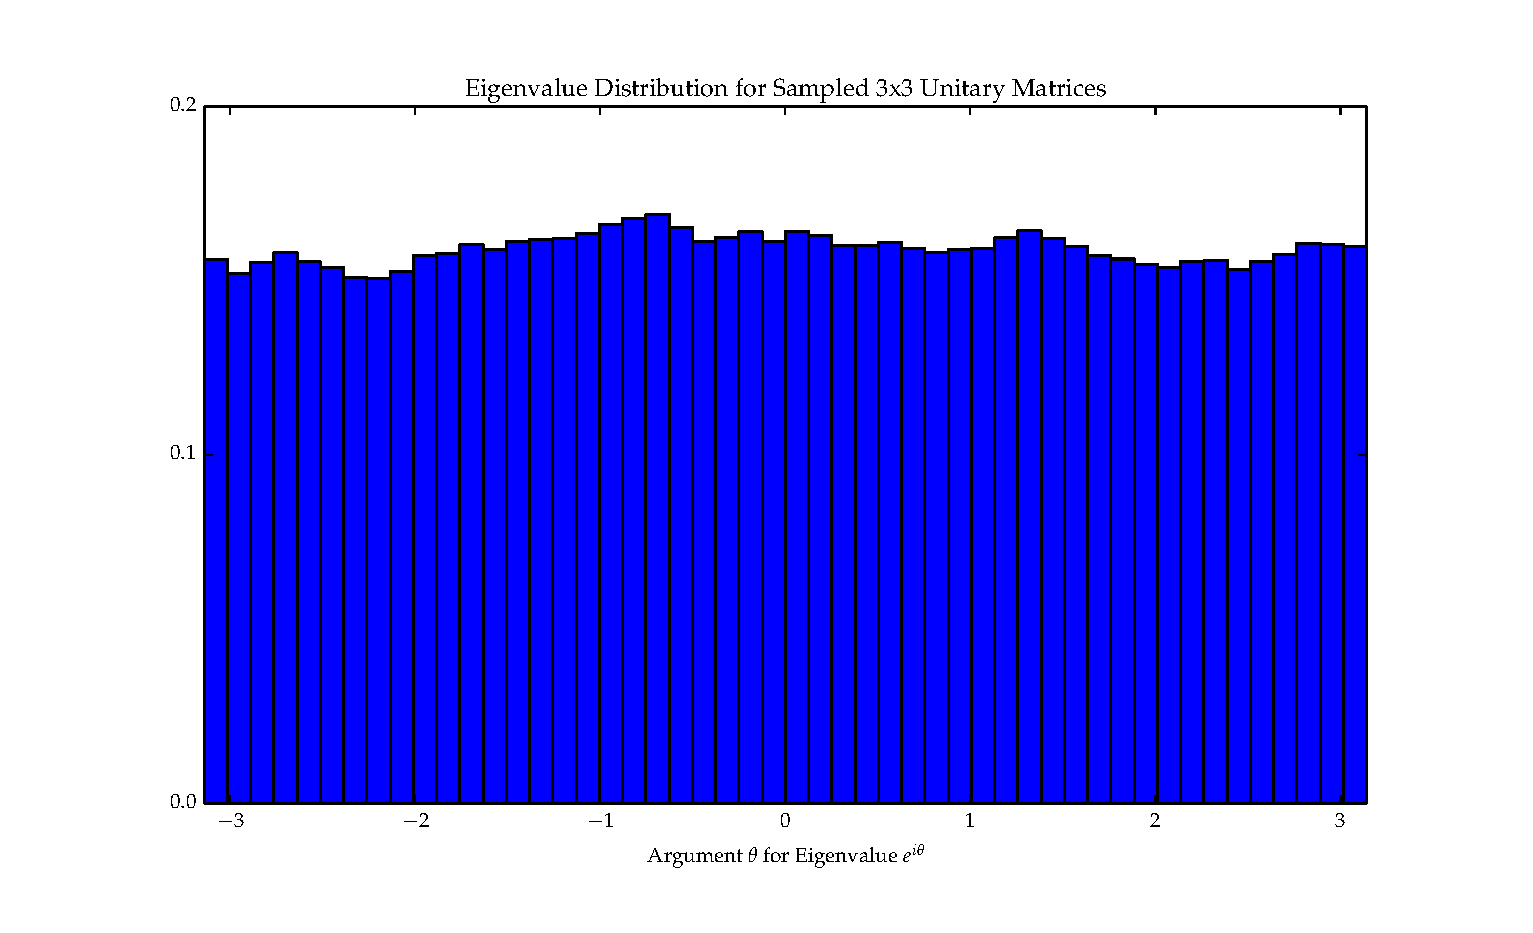
\includegraphics[scale=0.6, angle=0]{images/unitary_3_hist.eps}
\caption{Empirical distribution of $3\times 3$ Unitary matrices is uniform.}
\label{fig:Uny3}
\end{figure}
Mezzadri outlines properties of random unitary matrices~\cite{Mezzadri2007}. In particular, a uniform distribution according to the Haar measure corresponds to a uniform sampling of of the arguments $\theta$ of the matrices eigenvalues. Using our scheme, $3,000,000$ samples were drawn for both $N = 3$ and $N = 10$. Figures~\ref{fig:Uny3} and~\ref{fig:Uny10} show the eigenvalue distribution of our sampled matrices to be uniform.  
\begin{figure}[ht]
\centering
  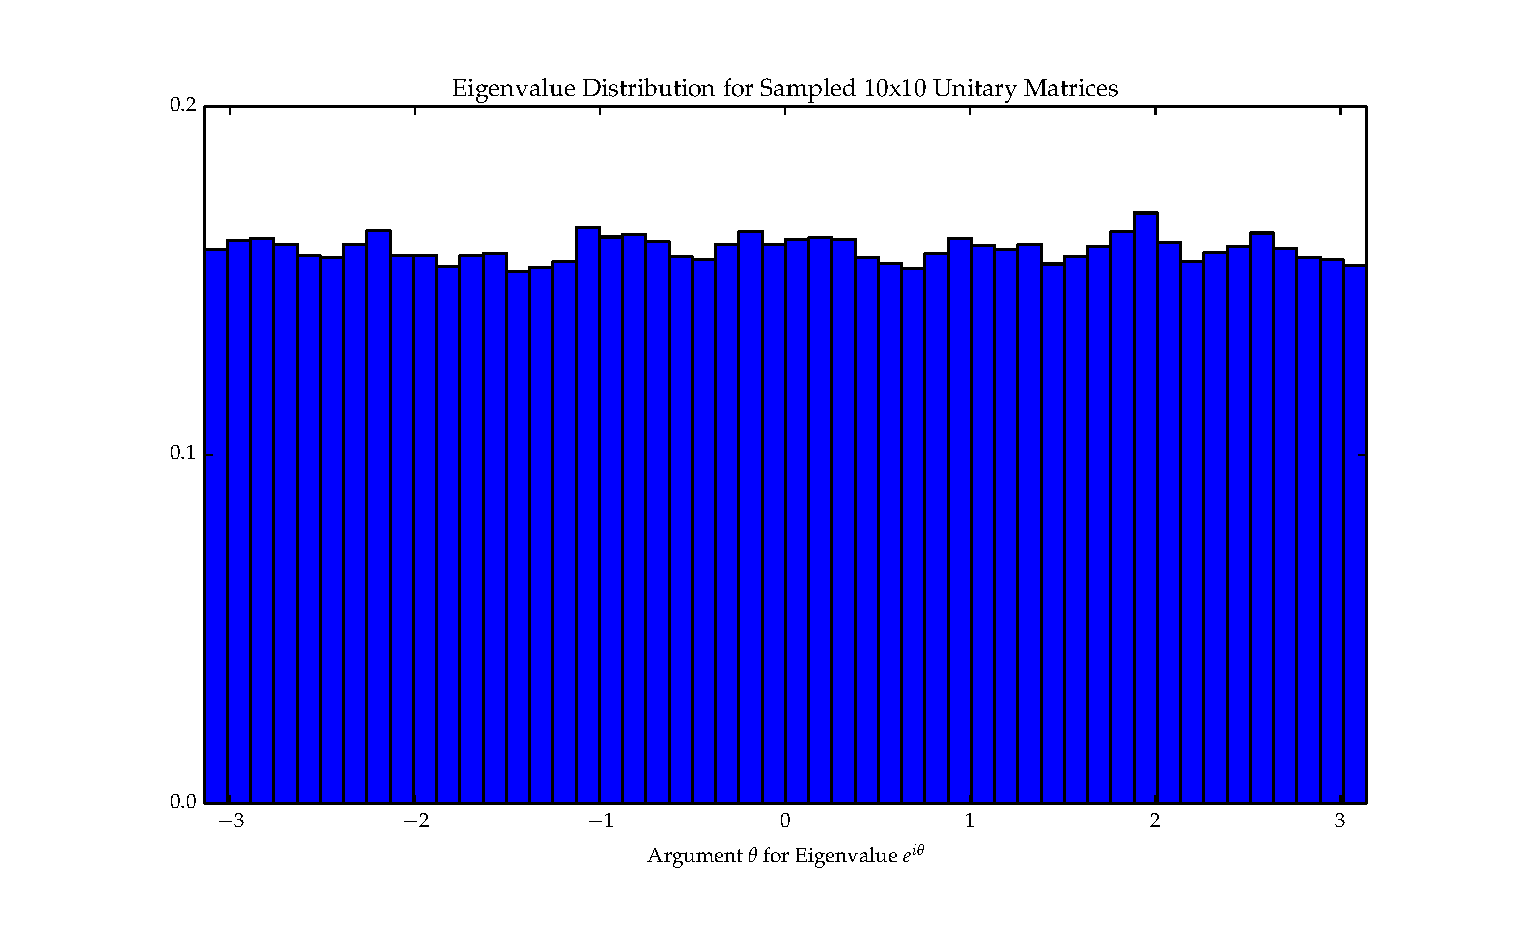
\includegraphics[scale=0.6, angle=0]{images/unitary_10_hist.eps}
\caption{Empirical distribution of $10\times 10$ Unitary matrices is uniform.}
\label{fig:Uny10}
\end{figure}

%--ellipsoid examples.?
 
\subsection{MBM on Geometric Configuration Spaces}
\label{ssc:MBMGCS}
As an initial test case of our Manifold Brownian Motion scheme on Building Game geometric configuration spaces, we first consider two simple triangle linkages. The first has two triangles linked together along a hinged edge. As seen in figure~\ref{fig:T2_diagram}, the linkage can be specified by the $3$-dimensional locations of four vertices, giving an ambient space of $\mathbbm{R}^3$. In addition to the six trivial degrees of freedom, this configuration also carries an internal degree of freedom corresponding to the dihedral angle formed at the hinged edge. 
\begin{figure}[ht]
\centering
  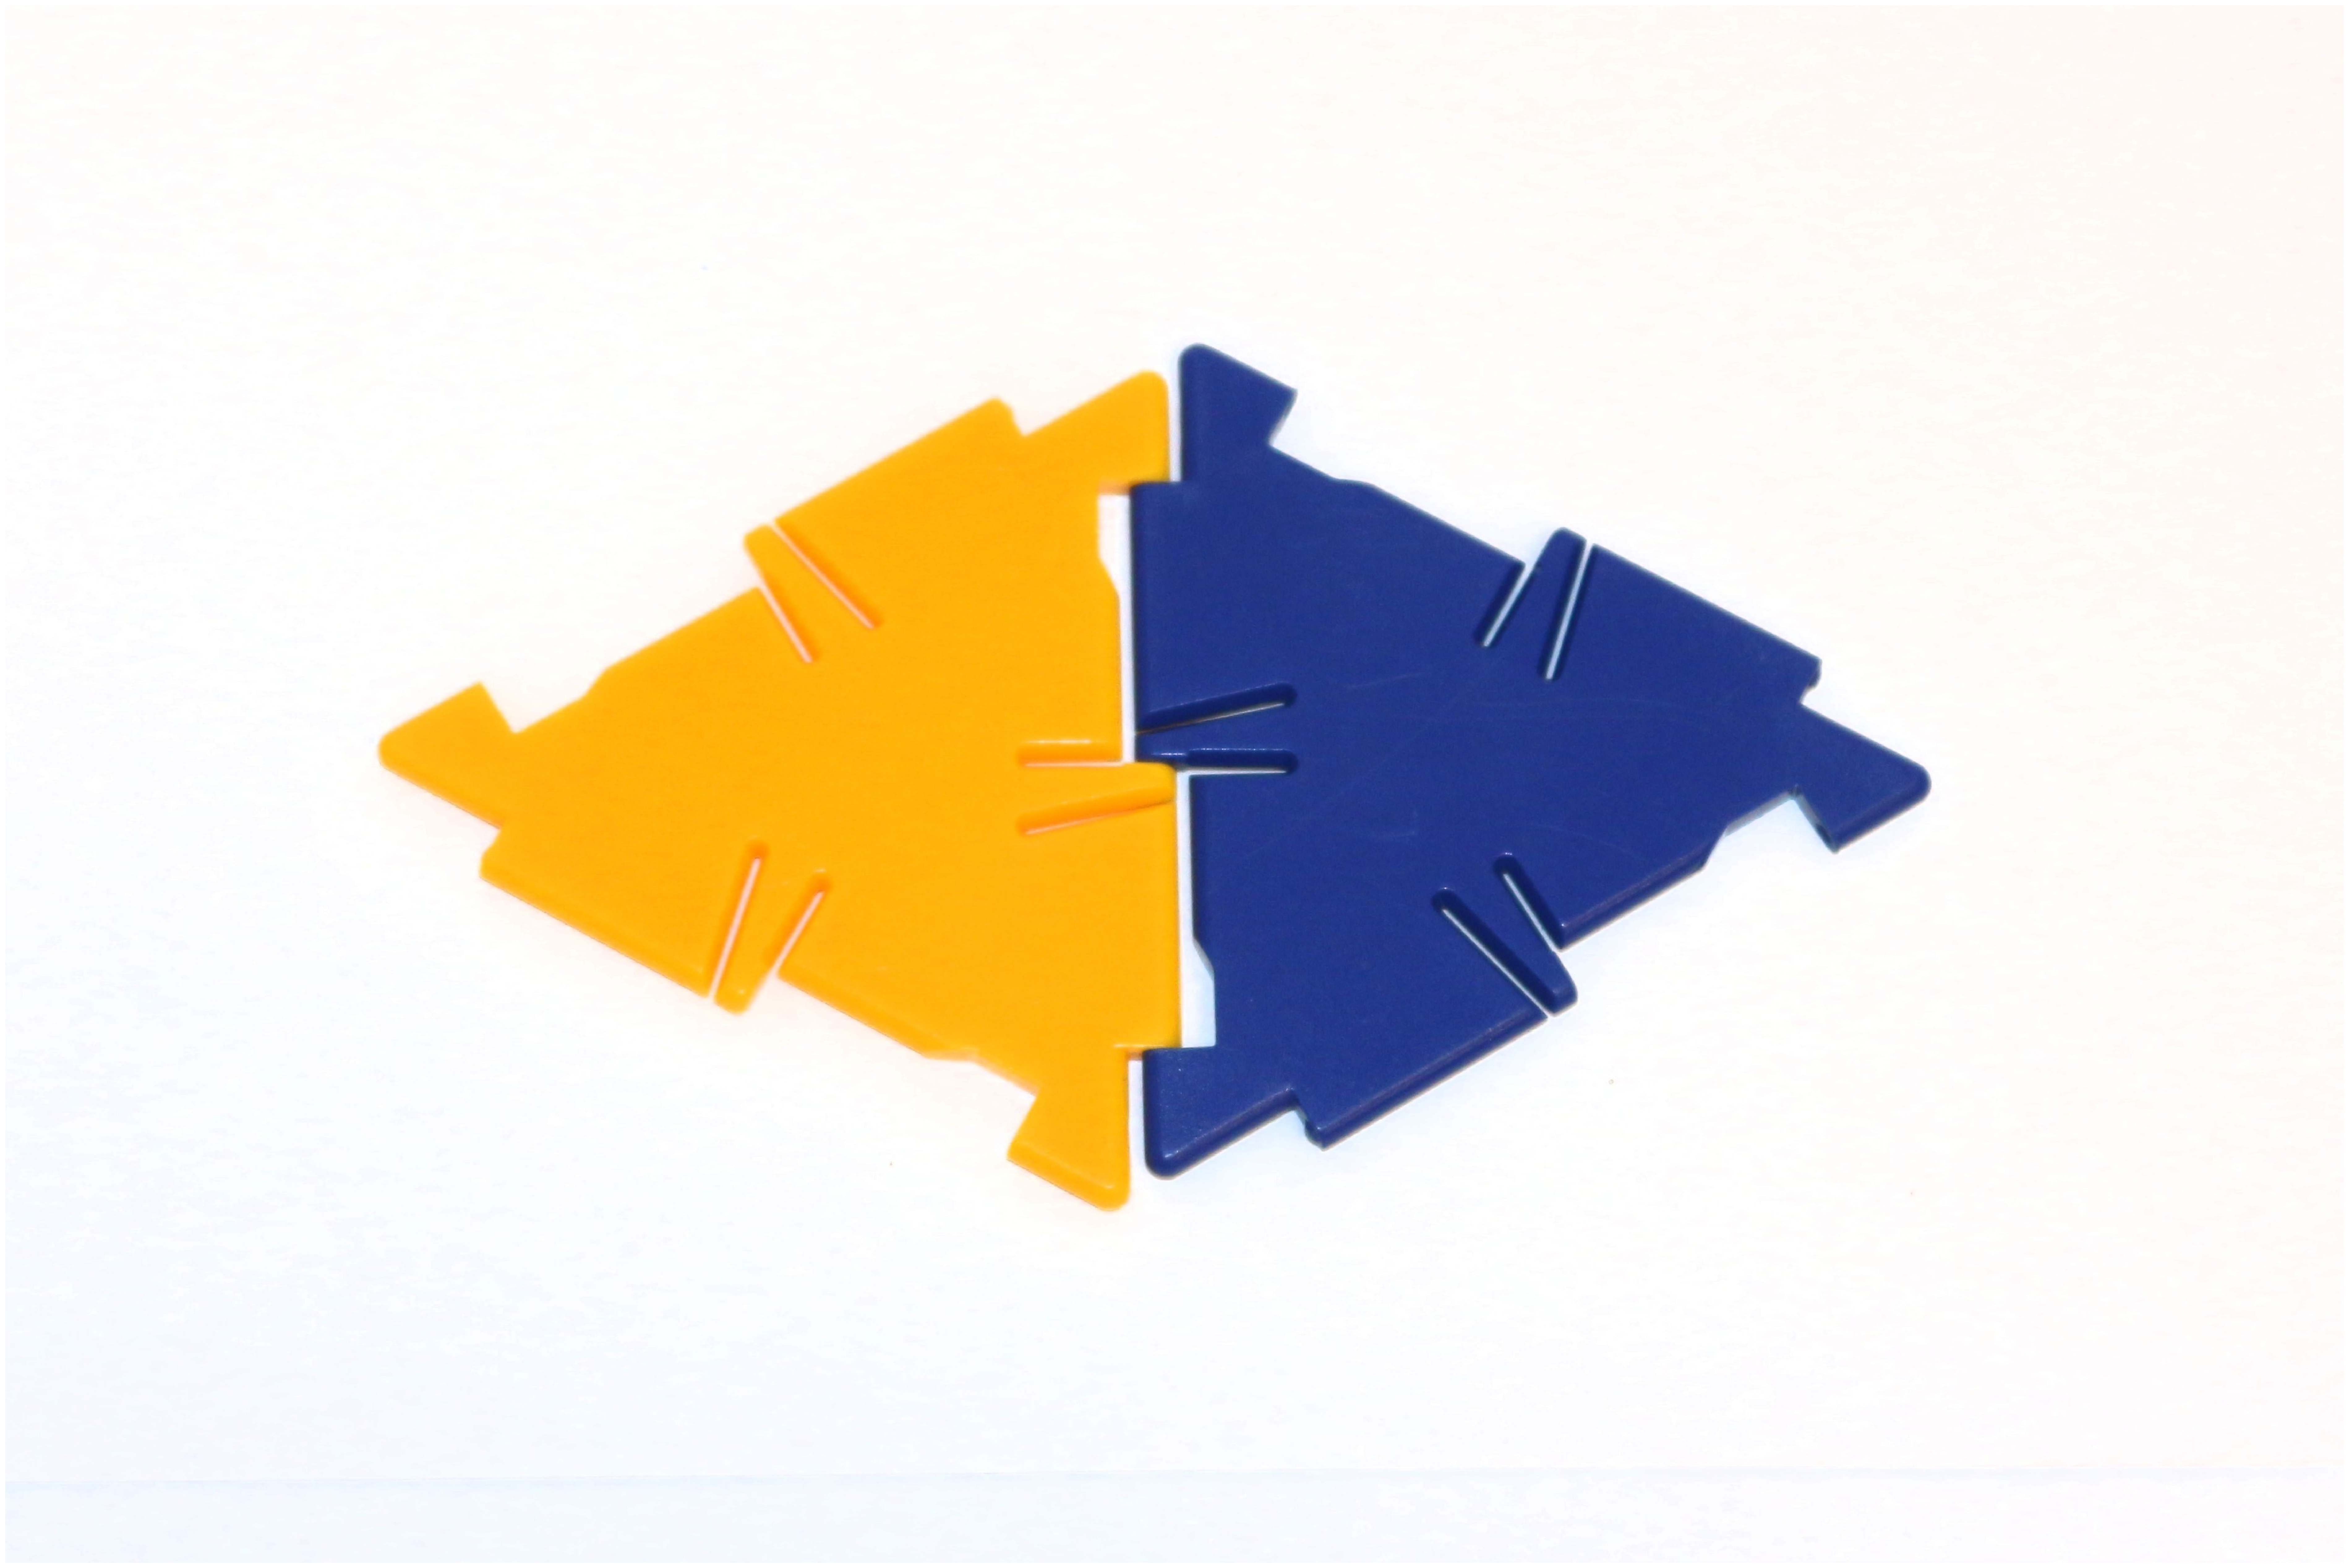
\includegraphics[scale=0.1]{images/T2_diagram.eps}
\caption{Two triangle linkage.}
\label{fig:T2_diagram}
\end{figure}
Figure~\ref{fig:T2_1} shows a histogram of this dihedral angle as sampled using out random walk scheme. Interestingly, the distribution is not uniform and appears to be of the form $\alpha_0 + \alpha_1\cos(\theta) + \alpha_2\cos(2\theta)$. 
\begin{figure}[ht]
\centering
  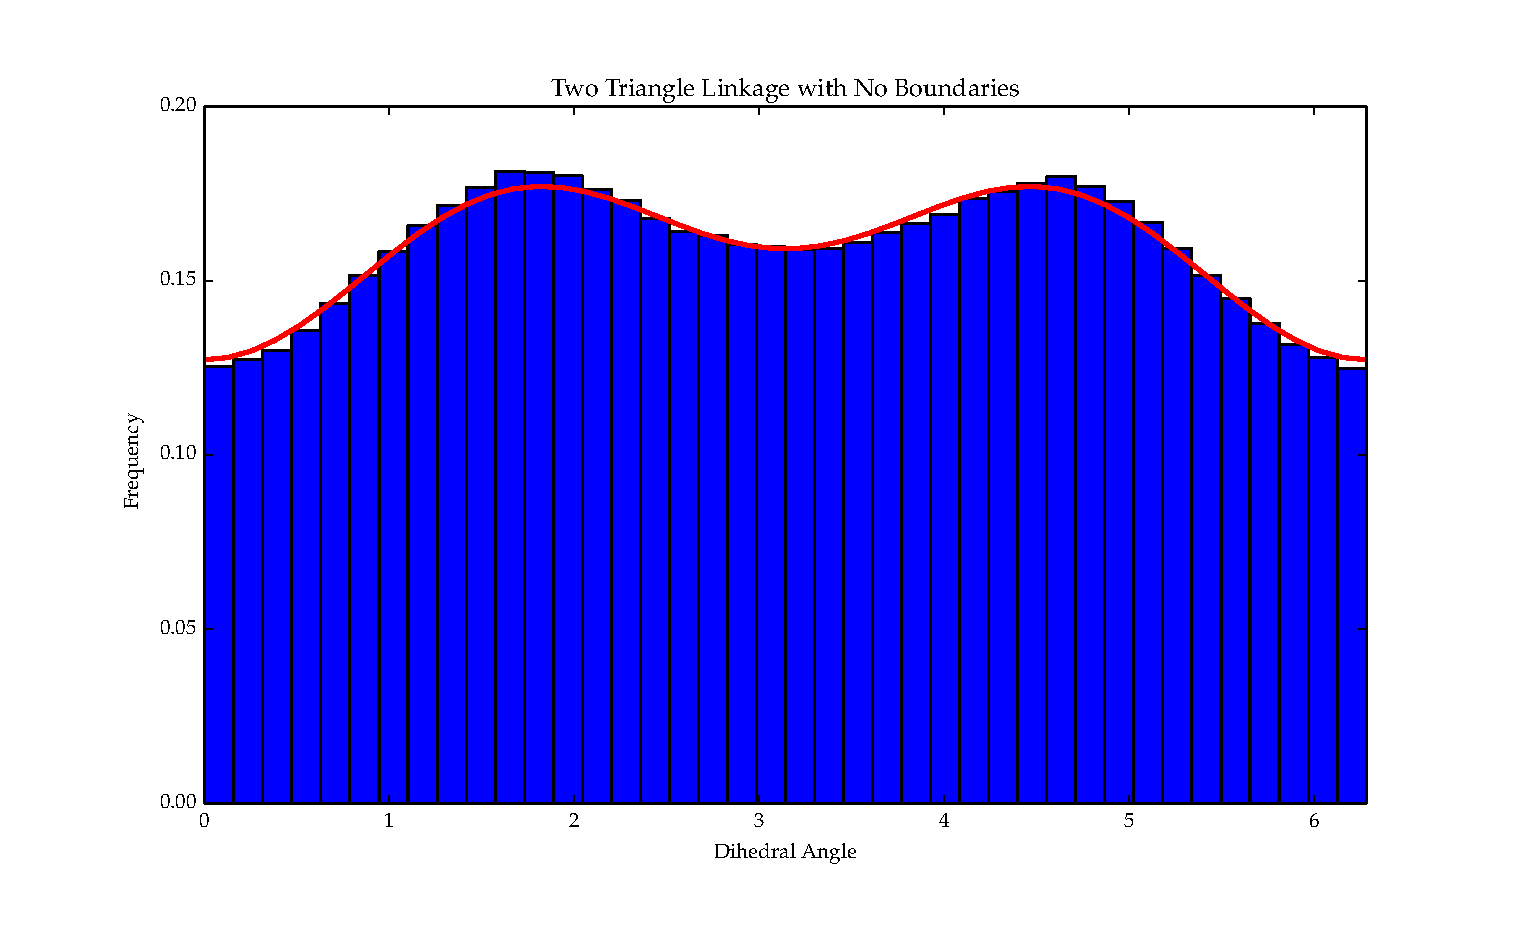
\includegraphics[scale=0.6]{images/T2_1.eps}
\caption{Histogram of the dihedral angle in sampled configurations of a two triangle linkage.}
\label{fig:T2_1}
\end{figure}

A second test case we consider is a linkage with three triangles. As depicted in figure~\ref{fig:T3_diagram}, the configuration is composed of an interior triangle connected along two of its edges to an additional two triangles and is parameterized by five vertices. 
\begin{figure}[ht]
\centering
  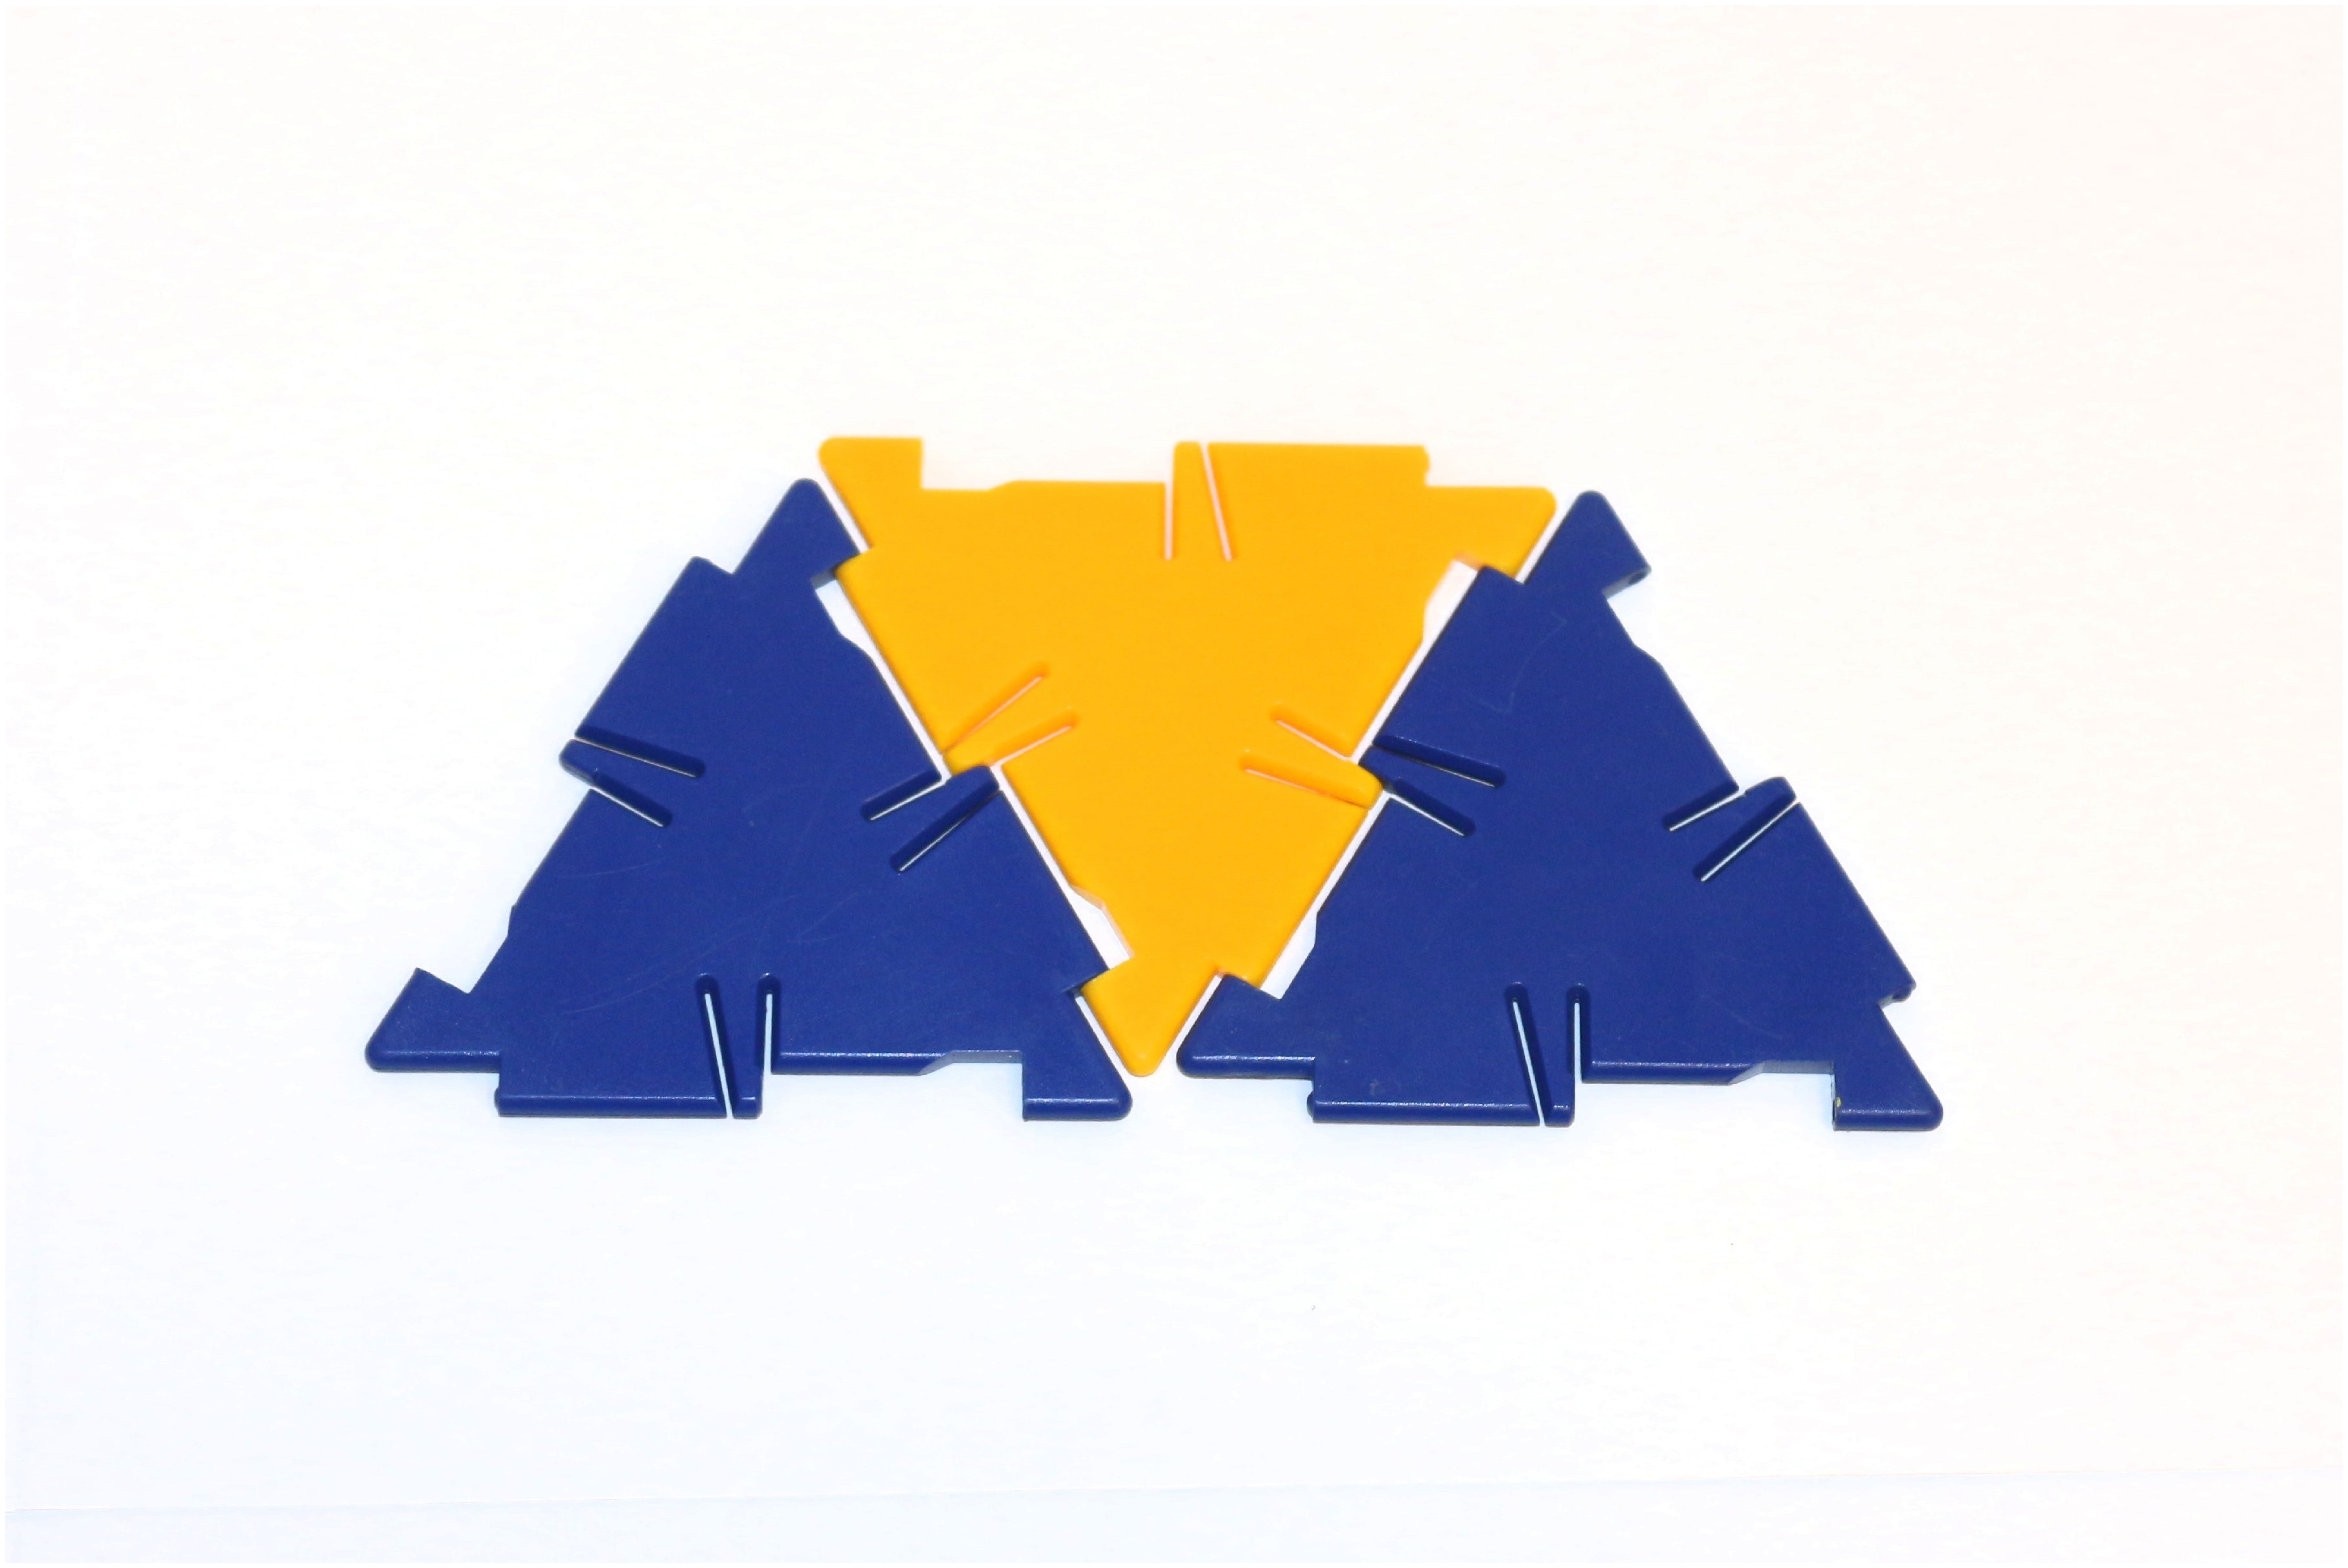
\includegraphics[scale=0.1]{images/T3_diagram.eps}
\caption{Three triangle linkage.}
\label{fig:T3_diagram}
\end{figure}
This configuration has two internal degrees of freedom, which are represented my the two dihedral angles. Figure~\ref{fig:T3_1} is a $2$-dimensional histogram of the dihedral angles sampled by our scheme. 
%As expected, the two dihedral angles are independent in the sense that individually their distributions look like that of the two triangle linkage.
\begin{figure}[ht]
\centering
  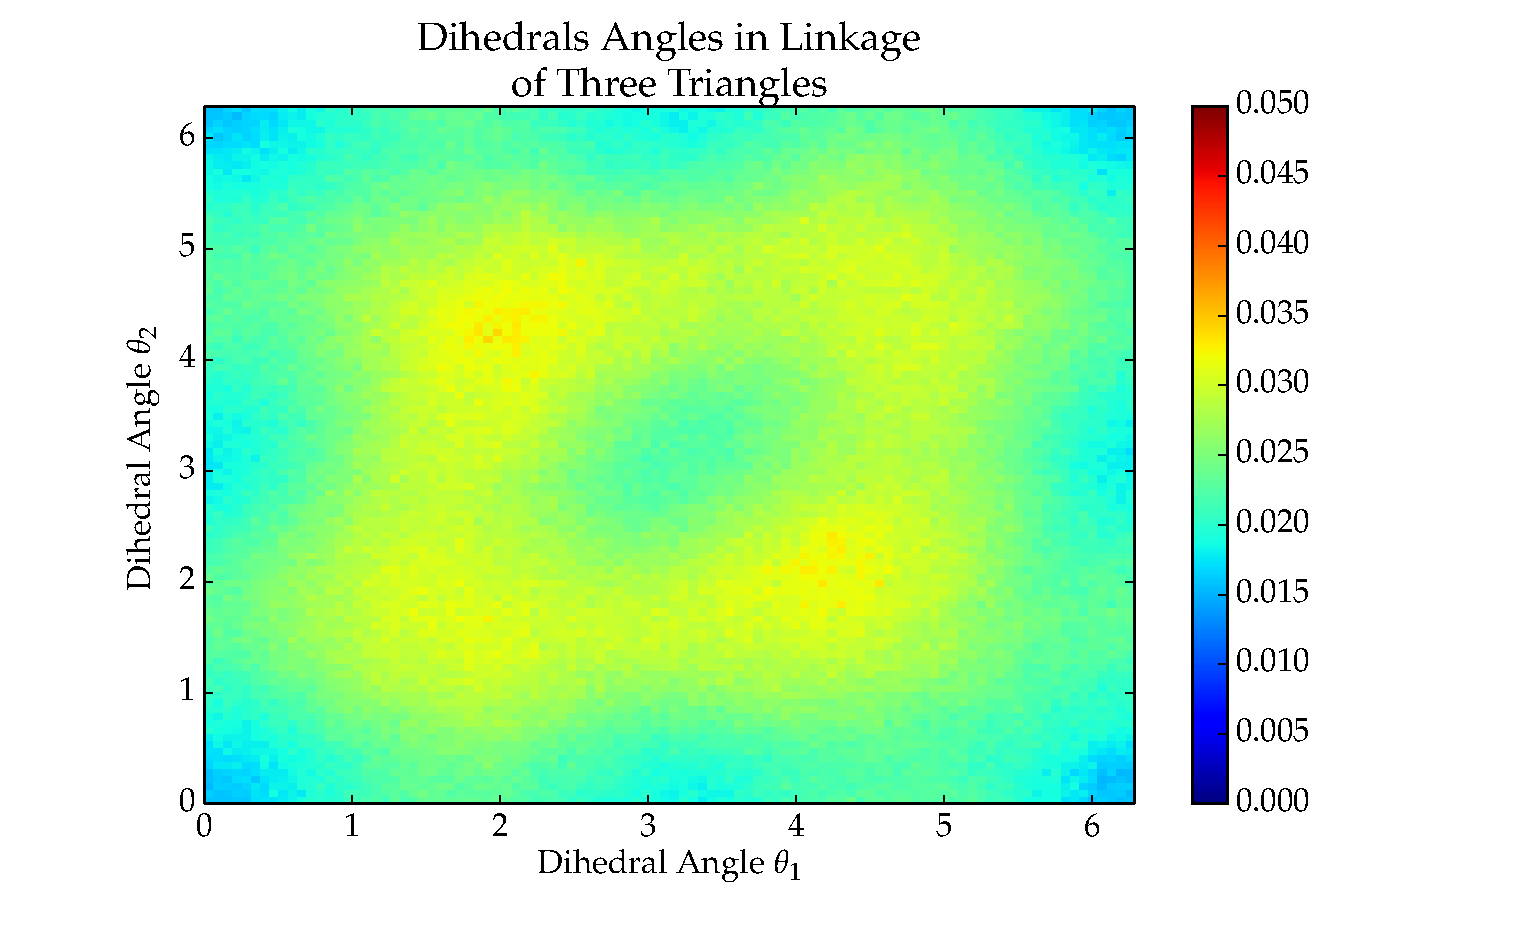
\includegraphics[scale=0.6]{images/T3_1_2D.eps}
\caption{Histogram of the dihedral angle in sampled configurations of a three triangle linkage.}
\label{fig:T3_1}
\end{figure}


\subsubsection{Fixing Trivial Degrees of Freedom}
From the two and three triangle linkage examples, we see that the sampling scheme does not sample the dihedral angles of the configuration uniformly. This was unexpected, but possible explained by the choice to not explicitly mod out the trivial rotational and translational degrees of freedom. 

The first apparent way of fixing the trivial degrees of freedom is to fix an individual face at a specific location. Without letting this face translate or rotate, we are also preventing these trivial degrees of freedom from entering the entire configuration. As seen in figure~\ref{fig:T2_3}, fixing of one of the faces in a two triangle linkage will give the dihedral angle a uniform distribution as hoped. 
\begin{figure}[ht]
\centering
  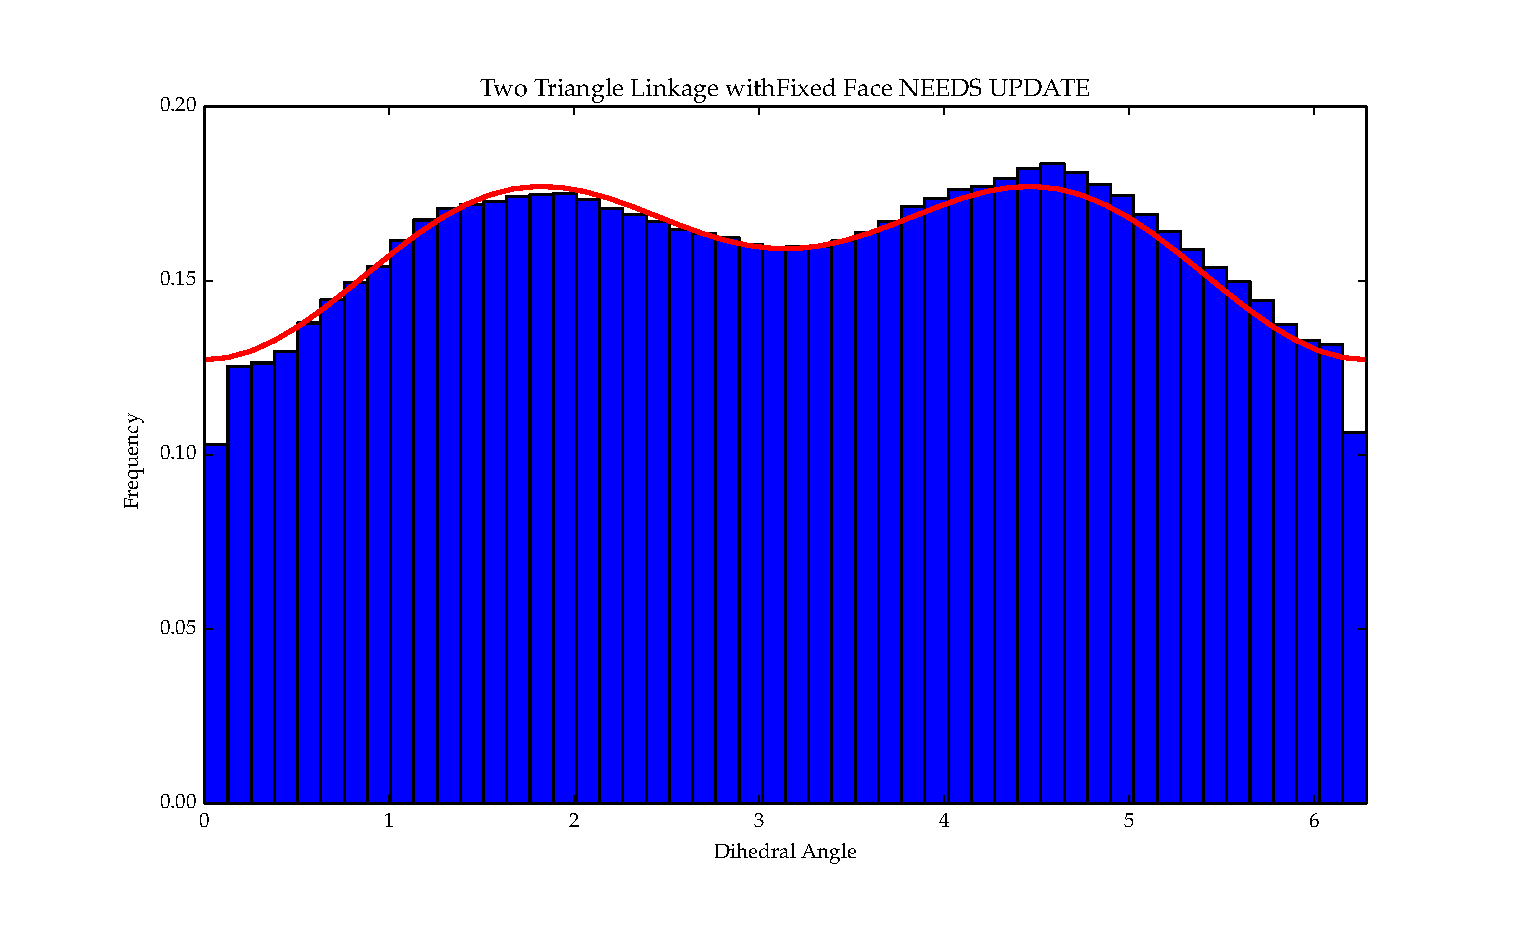
\includegraphics[scale=0.6]{images/T2_3.eps}
\caption{Two triangle linkage with one face fixed.}
\label{fig:T2_3}
\end{figure}
However, when we consider the three triangle linkage, there are two choices we have; we can either fix on of the outside triangles or we can fix the interior face. As seen in figure~\ref{fig:T3_3}, if we fix the interior triangle, the distribution we observe will be uniform. However, if we choose to fix an exterior triangle, the dihedral angle between the fixed triangle and the interior triangle  will be uniformly sampled, but the other dihedral will not have a uniform distribution. Seen in figure~\ref{fig:T3_4}, the distribution of this second dihedral angle appears to be the sum of trigonometric functions.
\begin{figure}[ht]
\centering
  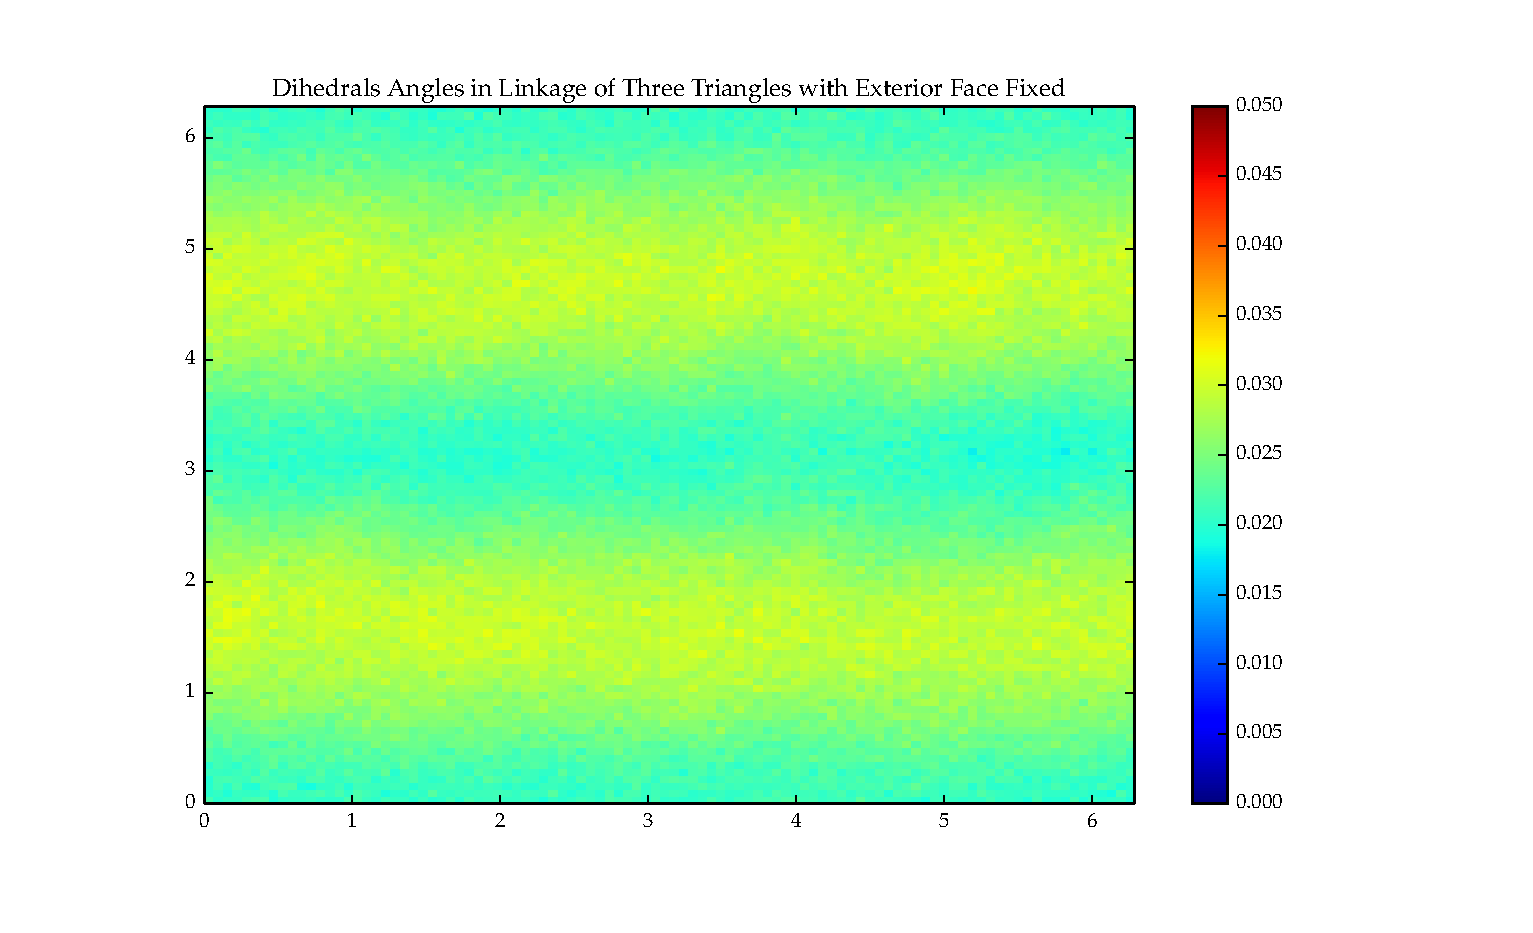
\includegraphics[scale=0.6]{images/T3_3_2D.eps}
\caption{Three triangle linkage with interior triangle fixed.}
\label{fig:T3_3}
  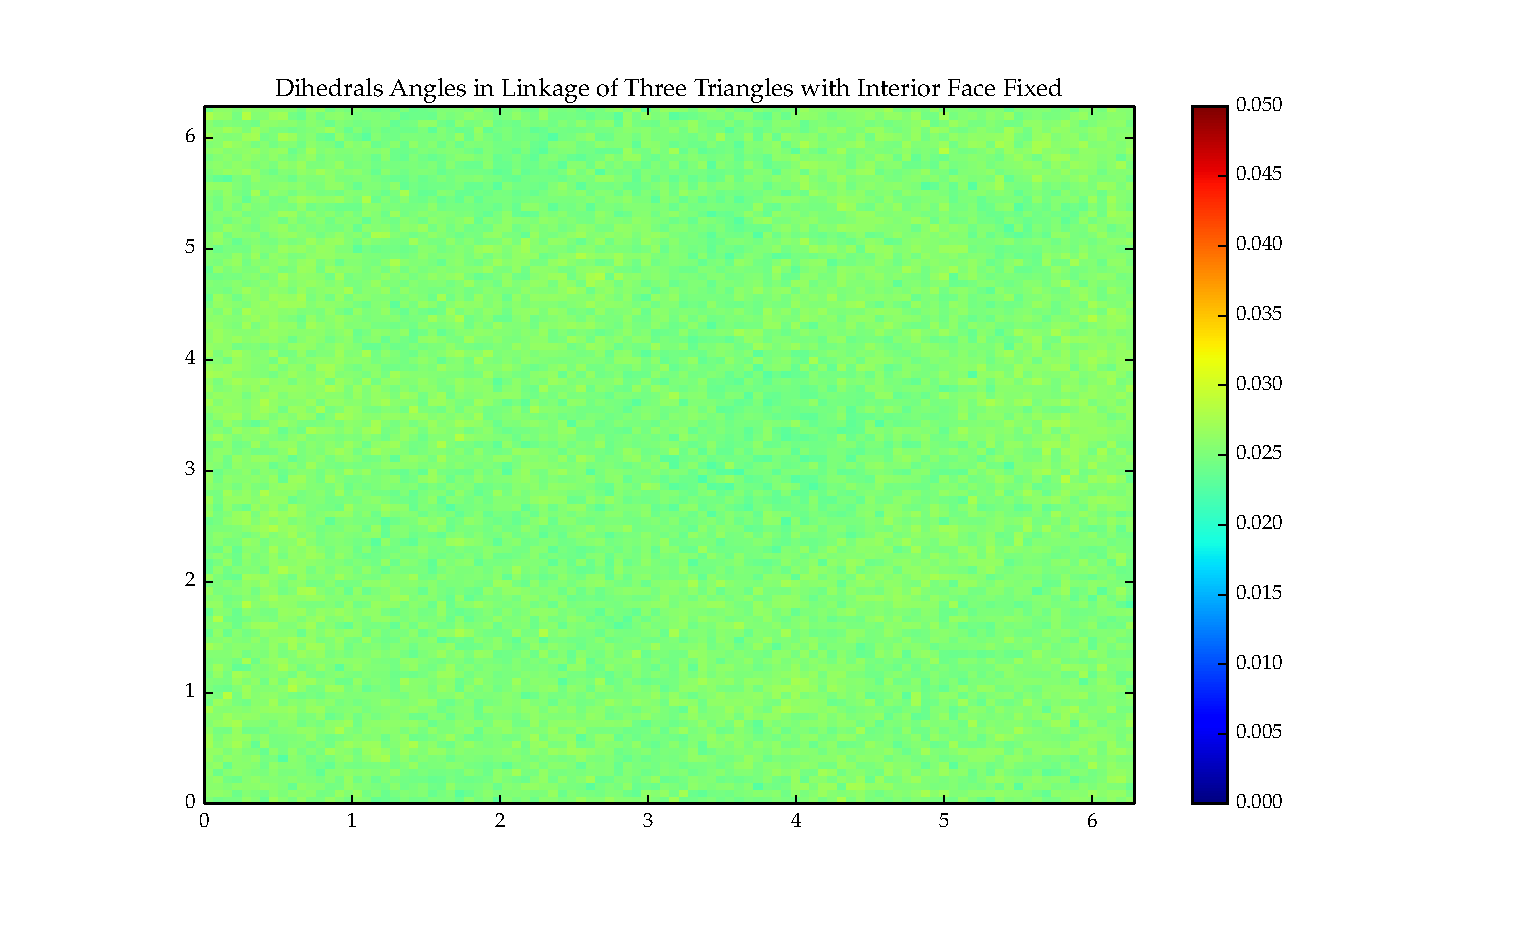
\includegraphics[scale=0.6]{images/T3_4_2D.eps}
\caption{Three triangle linkage with exterior triangle fixed.}
\label{fig:T3_4}
\end{figure}
This poses a bit of a problem. If the choice of face to fix affects the resulting distribution, then we must have justification for selecting one face over another. Since a clear reasoning for this choice is not apparent--especially in the case of an arbitrary linkage--we look to other methods for fixing the trivial degrees of freedom that the system has. 

As mentioned in section~\ref{ssc:RemTrivDoF}, one way of fixing the translational degrees of freedom is to fix the center of mass of the configuration. This method does not have the issue of the fixed face approach, but it also does not address the rotational degrees of freedom. From figure~\ref{fig:T2_4}, however, we see that fixing the center of mass does not result in a uniform sampling of the dihedral angle in a two triangle linkage. Thus, we account for the rotational degrees of freedom separately.  
\begin{figure}[ht]
\centering
  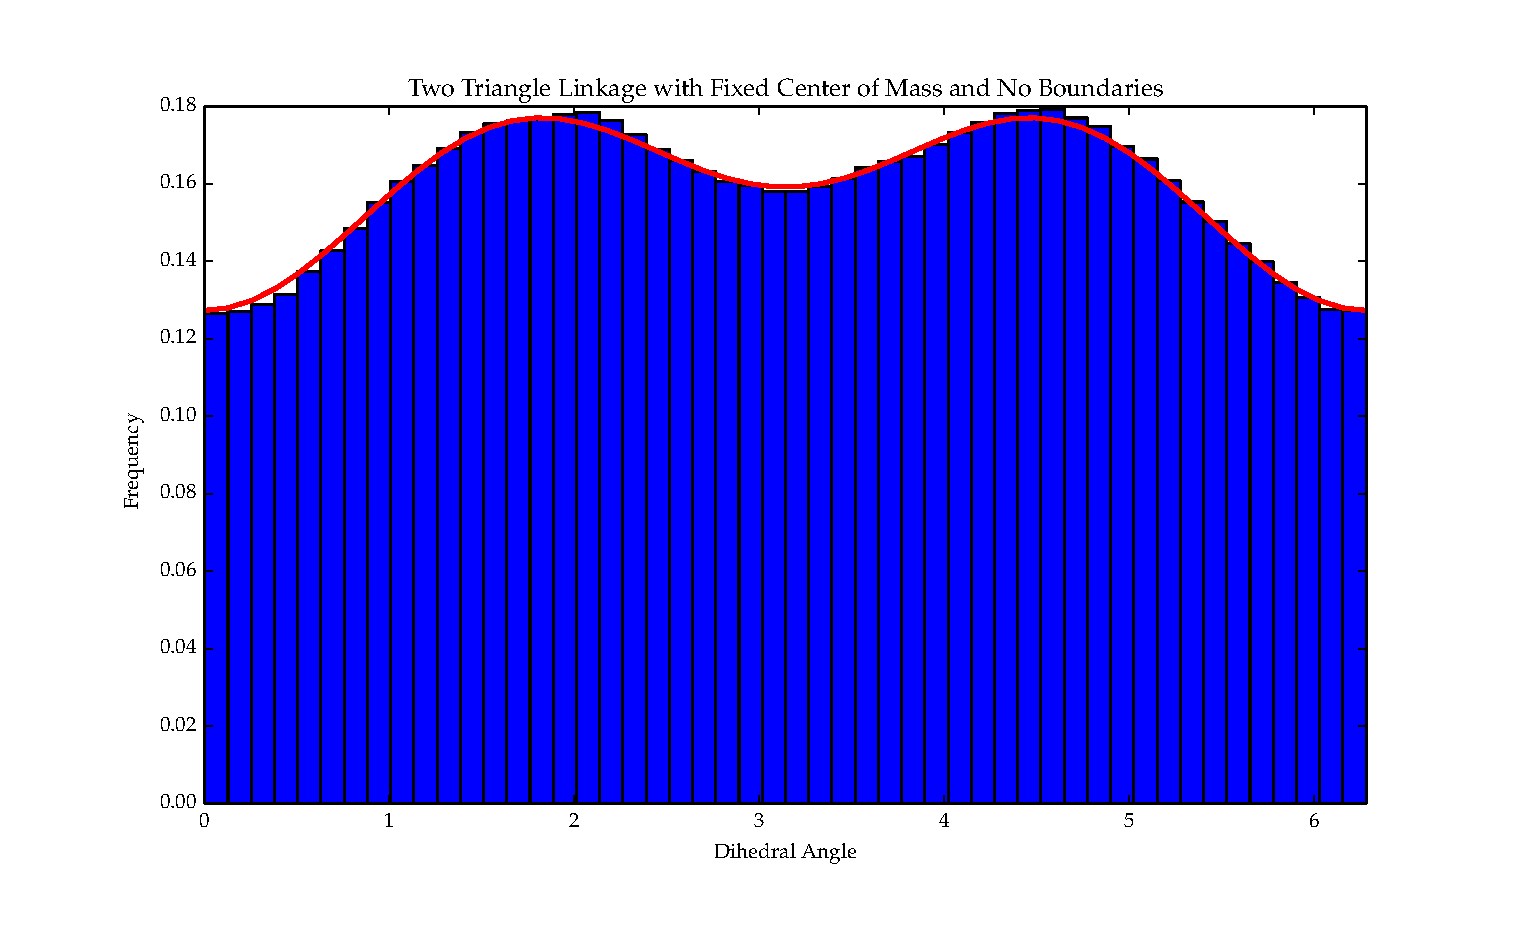
\includegraphics[scale=0.6]{images/T2_4.eps}
\caption{Sampling of two triangle linkage with fixed center of mass.}
\label{fig:T2_4}
\end{figure}

\begin{figure}[ht]
\centering
  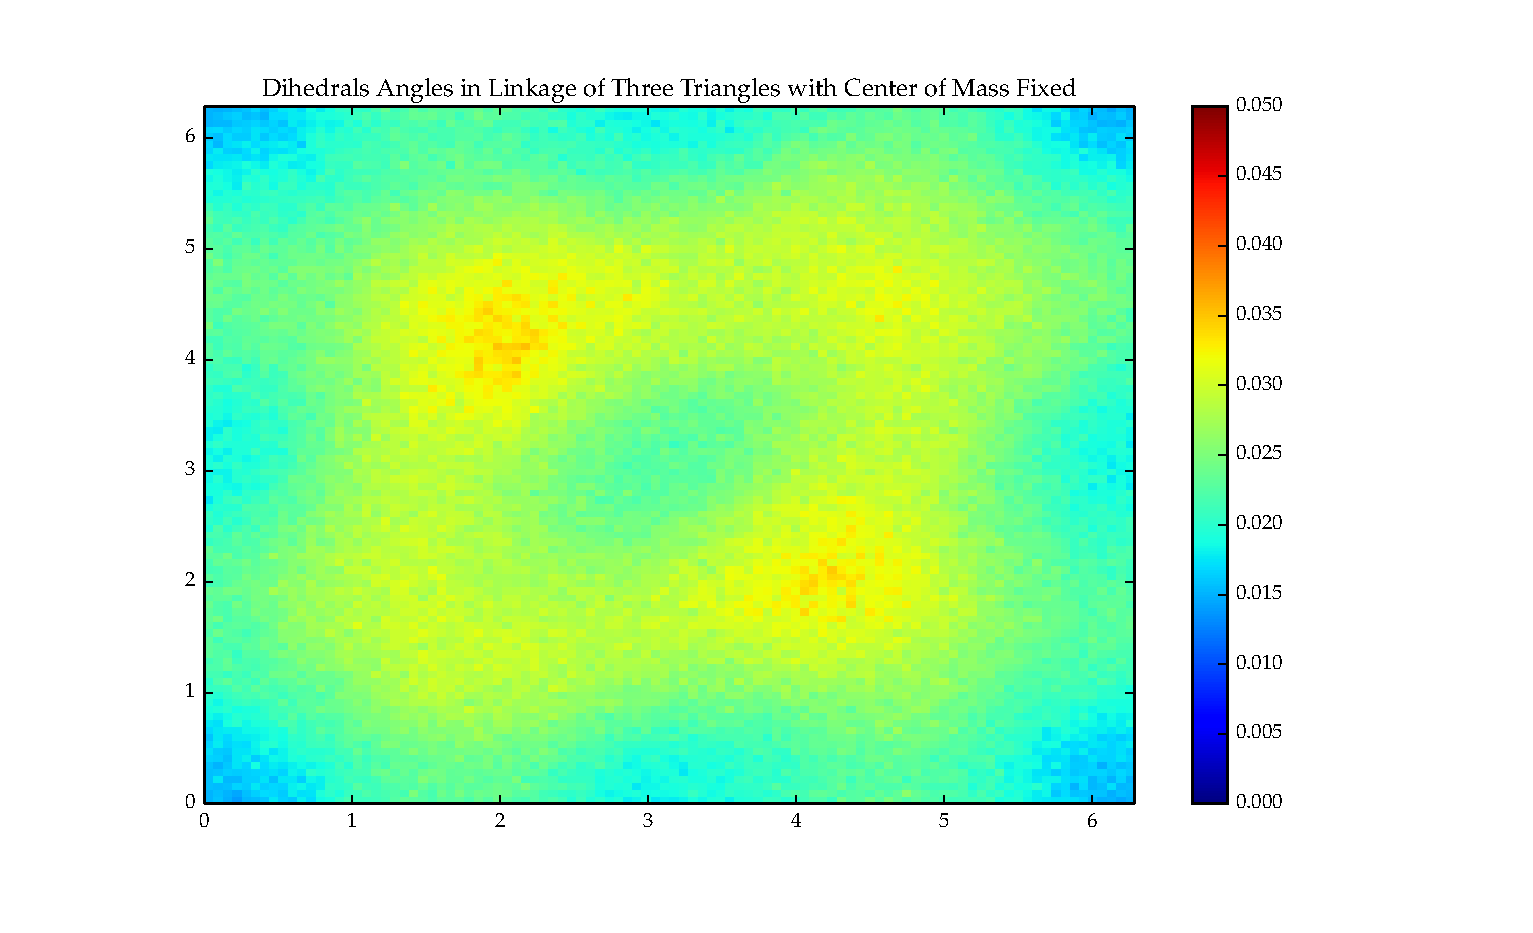
\includegraphics[scale=0.6]{images/T3_5_2D.eps}
\caption{Sampling of three triangle linkage with fixed center of mass.}
\label{fig:T3_5}
\end{figure}

Now, to address rotations, we seek to find the three dimensional subspace of the tangent space and restrict our random walk to the space orthogonal to these rotational directions. Since such a step in the tangent space is then projected to the manifold, some rotation may occur in the projection step. To account for this, we must add a correction step that rotates the configuration back to its original frame of reference. 

We treat our constraint space as the product of the special orthogonal group (rotations) and an algebraic variety corresponding to the remaining degrees of freedom $\mathcal{M} = SO(3) \times \tilde{\mathcal{M}}$. For every non-singular $z \in \mathcal{M}$ we notice that there is a local diffeomorphism from $\mathcal{M}$ to $SO(3) \times \tilde{\mathcal{M}}$. Using this knowledge, we aim to find local coordinates $Q \in SO(3)$ and $\tilde{z} \in \tilde{\mathcal{M}}$ such that the tangent space $\mathcal{T}_z\mathcal{M} = \mathcal{T}_QSO(3) \times \mathcal{T}_{\tilde{z}}\tilde{\mathcal{M}}$. Since we already have a method for deriving $\mathcal{T}_z\mathcal{M}$, the goal now is to decompose this tangent space into the two orthogonal subspaces corresponding to the rotational and internal degrees of freedom.

Since $z = (v^1, v^2, \dots, v^N)$ for $v^i \in \mathbbm{R}^3$, the rotation by a $Q \in SO(3)$ is really the vertex-wise rotation $\bar{Q}z = (Qv^1, Qv^2, \dots, Qv^N)$. In the case of $Q = I$ the tangent directions are generated by the skew-symmetric matrices. A basis for the skew-symmetric matrices is given by 
\begin{align}
\textswab{e}_1 &= \begin{pmatrix} 0 & 1 & 0 \\ -1 & 0 & 0 \\ 0 & 0 & 0  \end{pmatrix} \\
\textswab{e}_2 &= \begin{pmatrix} 0 & 0 & 1 \\ 0 & 0 & 0 \\ -1 & 0 & 0  \end{pmatrix} \\
\textswab{e}_3 &= \begin{pmatrix} 0 & 0 & 0 \\ 0 & 0 & 1 \\ 0 & -1 & 0  \end{pmatrix}.
\end{align}
Thus, in the case of $Q=I$ we can represent the rotational directions of the tangent space as $\mathcal{T}_ISO(3) = \text{span}(w_1, w_2, w_3)$ where the bases $w_1, w_2, w_3$ are defined by 
\begin{align}
w_1 &= (\textswab{e}_1v^1, \textswab{e}_1v^2, \dots, \textswab{e}_1v^N) \\
w_2 &= (\textswab{e}_2v^1, \textswab{e}_2v^2, \dots, \textswab{e}_2v^N) \\
w_3 &= (\textswab{e}_3v^1, \textswab{e}_3v^2, \dots, \textswab{e}_3v^N).
\end{align}

With this formulation, we can alter our method for finding the bases of the tangent space from theorem~\ref{thm:Qbases} to get the decomposition we desire. Specifically, setting 
$$\tilde{A} = \left[C^T(z) (w_1, w_2, w_3) \tilde{B} \right]$$
where $B \in \mathbbm{R}^{n\times (m-3)}$ is again random and taking the QR decomposition will give us 
$$\tilde{A} = \left[Q^{(1)} Q^{(2)}_{rot} Q^{(2)}_{int}\right]R.$$
As before, $Q^{(2)} = \left[Q^{(2)}_{rot} Q^{(2)}_{int} \right]$ is a basis for $\mathcal{T}_z\mathcal{M}$, but we will also have $Q^{(2)}_{rot}$ as a basis for the rotational directions $\mathcal{T}_ISO(3)$ and $Q^{(2)}_{int}$ as a basis for the remaining internal tangent directions $\mathcal{T}_{\tilde{z}}\tilde{\mathcal{M}}$. Thus by modifying our 
random walk routine to sample from the directions of $Q_{int}^{(2)}$, we will fix the rotation of the proposed step in the tangent space.

Two issues must still be addressed. First, we have assumed that that the local rotation coordinate $Q$ is the identity. Additionally, even though our step in tangent space does not contain any of the rotational directions, when it is projected back to the constraint space, some rotation may occur. We address these two issues simultaneously in the form of a correction step after the projection has been made. To do this, the configuration is simply rotated back to its original frame of reference using the Kabsch algorithm which finds the optimal rotation by which to match two sets of points in three dimensions~\cite{Kabsch}. The implicit assumption here is that if we have bad a sufficiently small random walk step, the resulting configuration will be close to the one at the previous step. Moreover, if $Q=I$ at the previous step, this rotation will bring the configuration back to the same frame of reference. 

Figure~\ref{fig:T2_5} shows the results for a sampling of configurations for the two triangle linkage. The distribution of dihedral angle is still not uniform, but takes the form of a simpler cosine function. 
\begin{figure}[ht]
\centering
  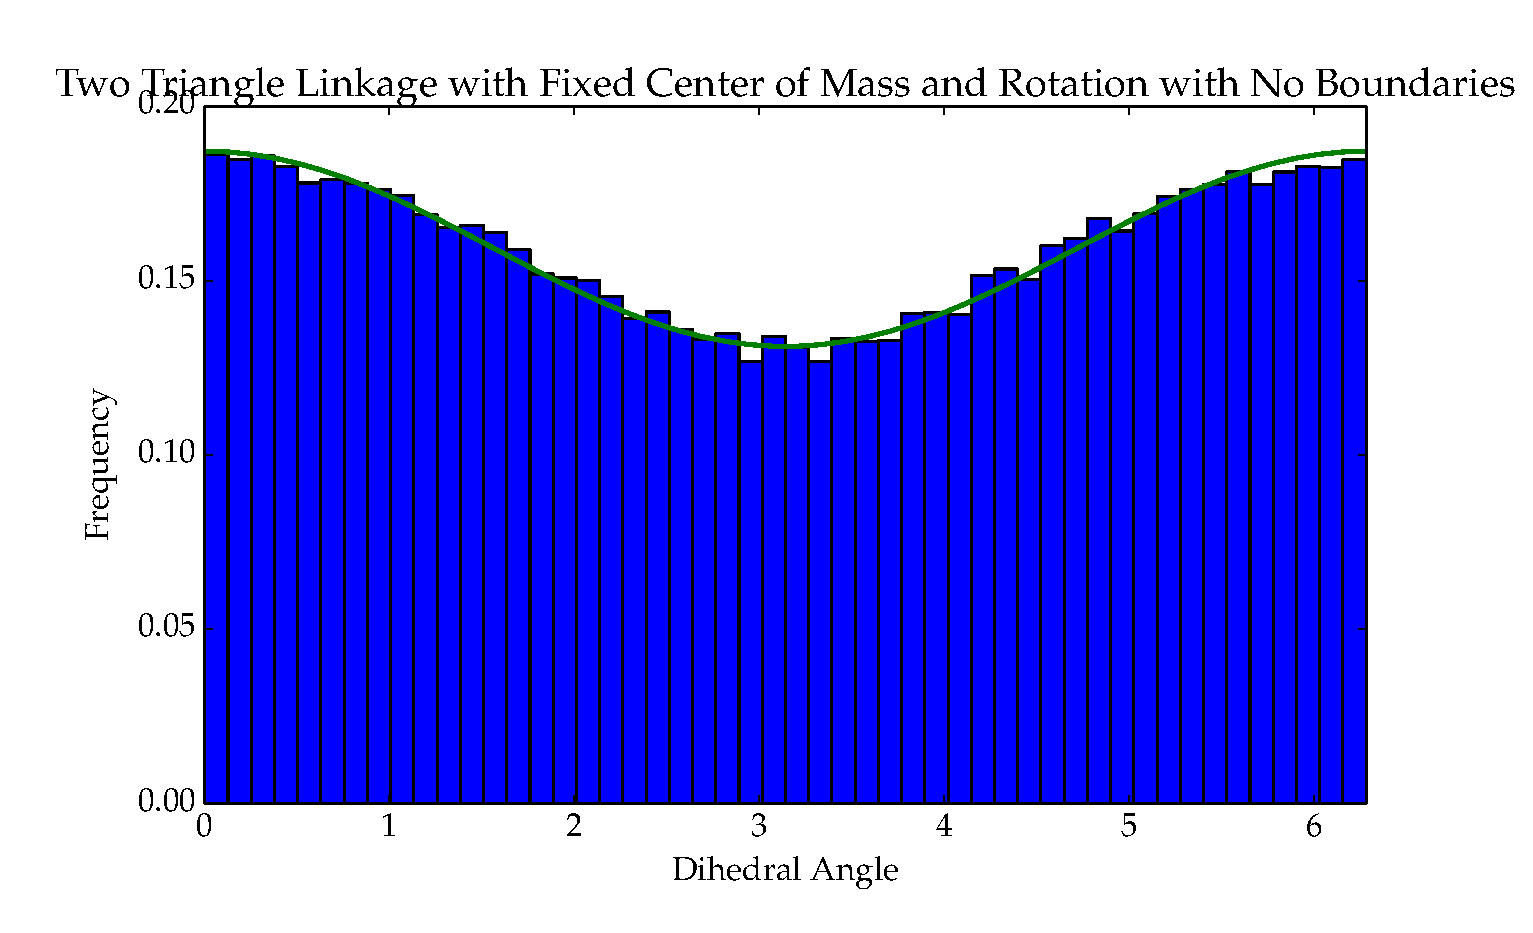
\includegraphics[scale=0.6]{images/T2_5.eps}
\caption{Sampling of two triangle linkage with fixed center of mass and rotations.}
\label{fig:T2_5}
\end{figure}
Similarly, the three triangle linkage also does not produce a uniform sampling of dihedral angles. As seen in figure~\ref{fig:T3_6}, the distribution is not the simple product of one-dimensional distributions. There are local maxima at $(0,0), (\frac{\pi}{3}, \frac{5\pi}{3})$, and $(\frac{5\pi}{3}, \frac{\pi}{3})$ With a local minima at $(\pi,\pi)$. 
\begin{figure}[ht]
\centering
  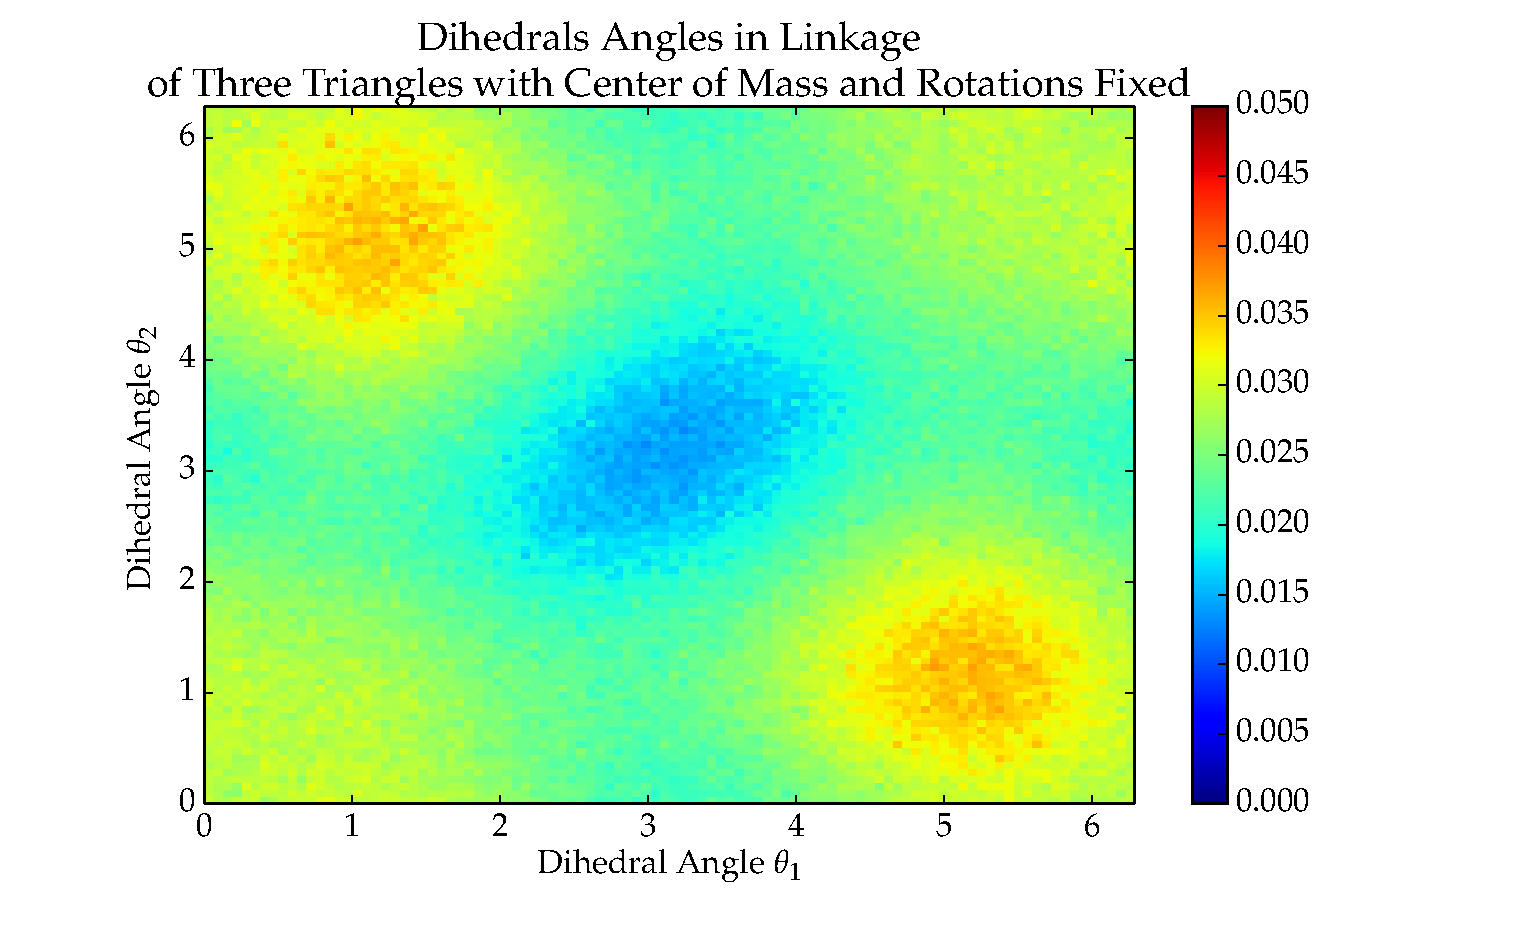
\includegraphics[scale=0.6]{images/T3_6_2D.eps}
\caption{Sampling of three triangle linkage with fixed center of mass and rotations.}
\label{fig:T3_6}
\end{figure}

\section{Manifold Reflected Brownian Motion}
In our sampling of Building Game geometric configurations, we see that many of the sampled configurations or Brownian motion paths do not make physical sense. For example, we do not prevent the triangles of the configuration from intersecting each other. Additionally, two faces attached by a hinge may pass through each other as the dihedral angle passes through zero. We introduce implicit boundaries to turn the manifold Brownian motion into a manifold reflected Brownian motion. With these added boundaries, the process will be prevented from entering nonphysical configurations, and represents a better sampling on configurations that coincide with the actual self-assembly processes we are attempting to model.

\subsection{Computational Scheme}

To sample from a reflected Brownian motion on the manifold, we use a rejection scheme that first generates a proposal configuration according to the previous random walk scheme. Using our implicit boundary function that simply returns true if a proposed configuration is valid (not self-intersecting), and false otherwise, we accept or reject the proposed configuration. This process repeats until a proposal is accepted. 

%\begin{figure}[ht]
%\centering
%\begin{algorithmic}
%\Do 
%\State $\hat{z} \gets$ proposal configuration using algorithm~\ref{alg:MBMRW}.
%\doWhile{$\hat{z}$ is self-intersecting}
%\State $z \gets \hat{z}$
%\end{algorithmic}
%\caption{Reflected Random Walk on $\mathcal{M}$}
%\end{figure}

\subsubsection{Self-Intersection Testing}

In order to compute our implicit self-intersection function at each step, we must ensure that no two triangles intersect. Thus, for an intermediate $[x]$, each function call requires that $\frac{1}{2}|x|(|x| - 1)$ pairs of triangle be tested for intersection. For the scheme to remain computationally feasible, it is imperative that these comparisons are carried out as efficiently as possible. We use an algorithm presented by M\"oller, which has been shown to be effective ~\cite{Möller97afast}.

%\begin{figure}[ht]
%\centering
%\begin{algorithmic}
%\State HI
%\end{algorithmic}
%\caption{Self Intersection Boundary}
%\end{figure} 

\subsection{Validation and Test Cases}

One way to test whether our rejection scheme has the properties that coincide with a reflected Brownian motion is to look at its distribution after a finite amount of time rather than only looking at long time statistics. In figure~\ref{fig:HCFin} we consider the case of a $d$-dimensional hyper-cube for $d = 2, 3, 4, 5$  and compare the distribution after a finite simulation time with the exact solution. 
\begin{figure}[ht]
\centering
  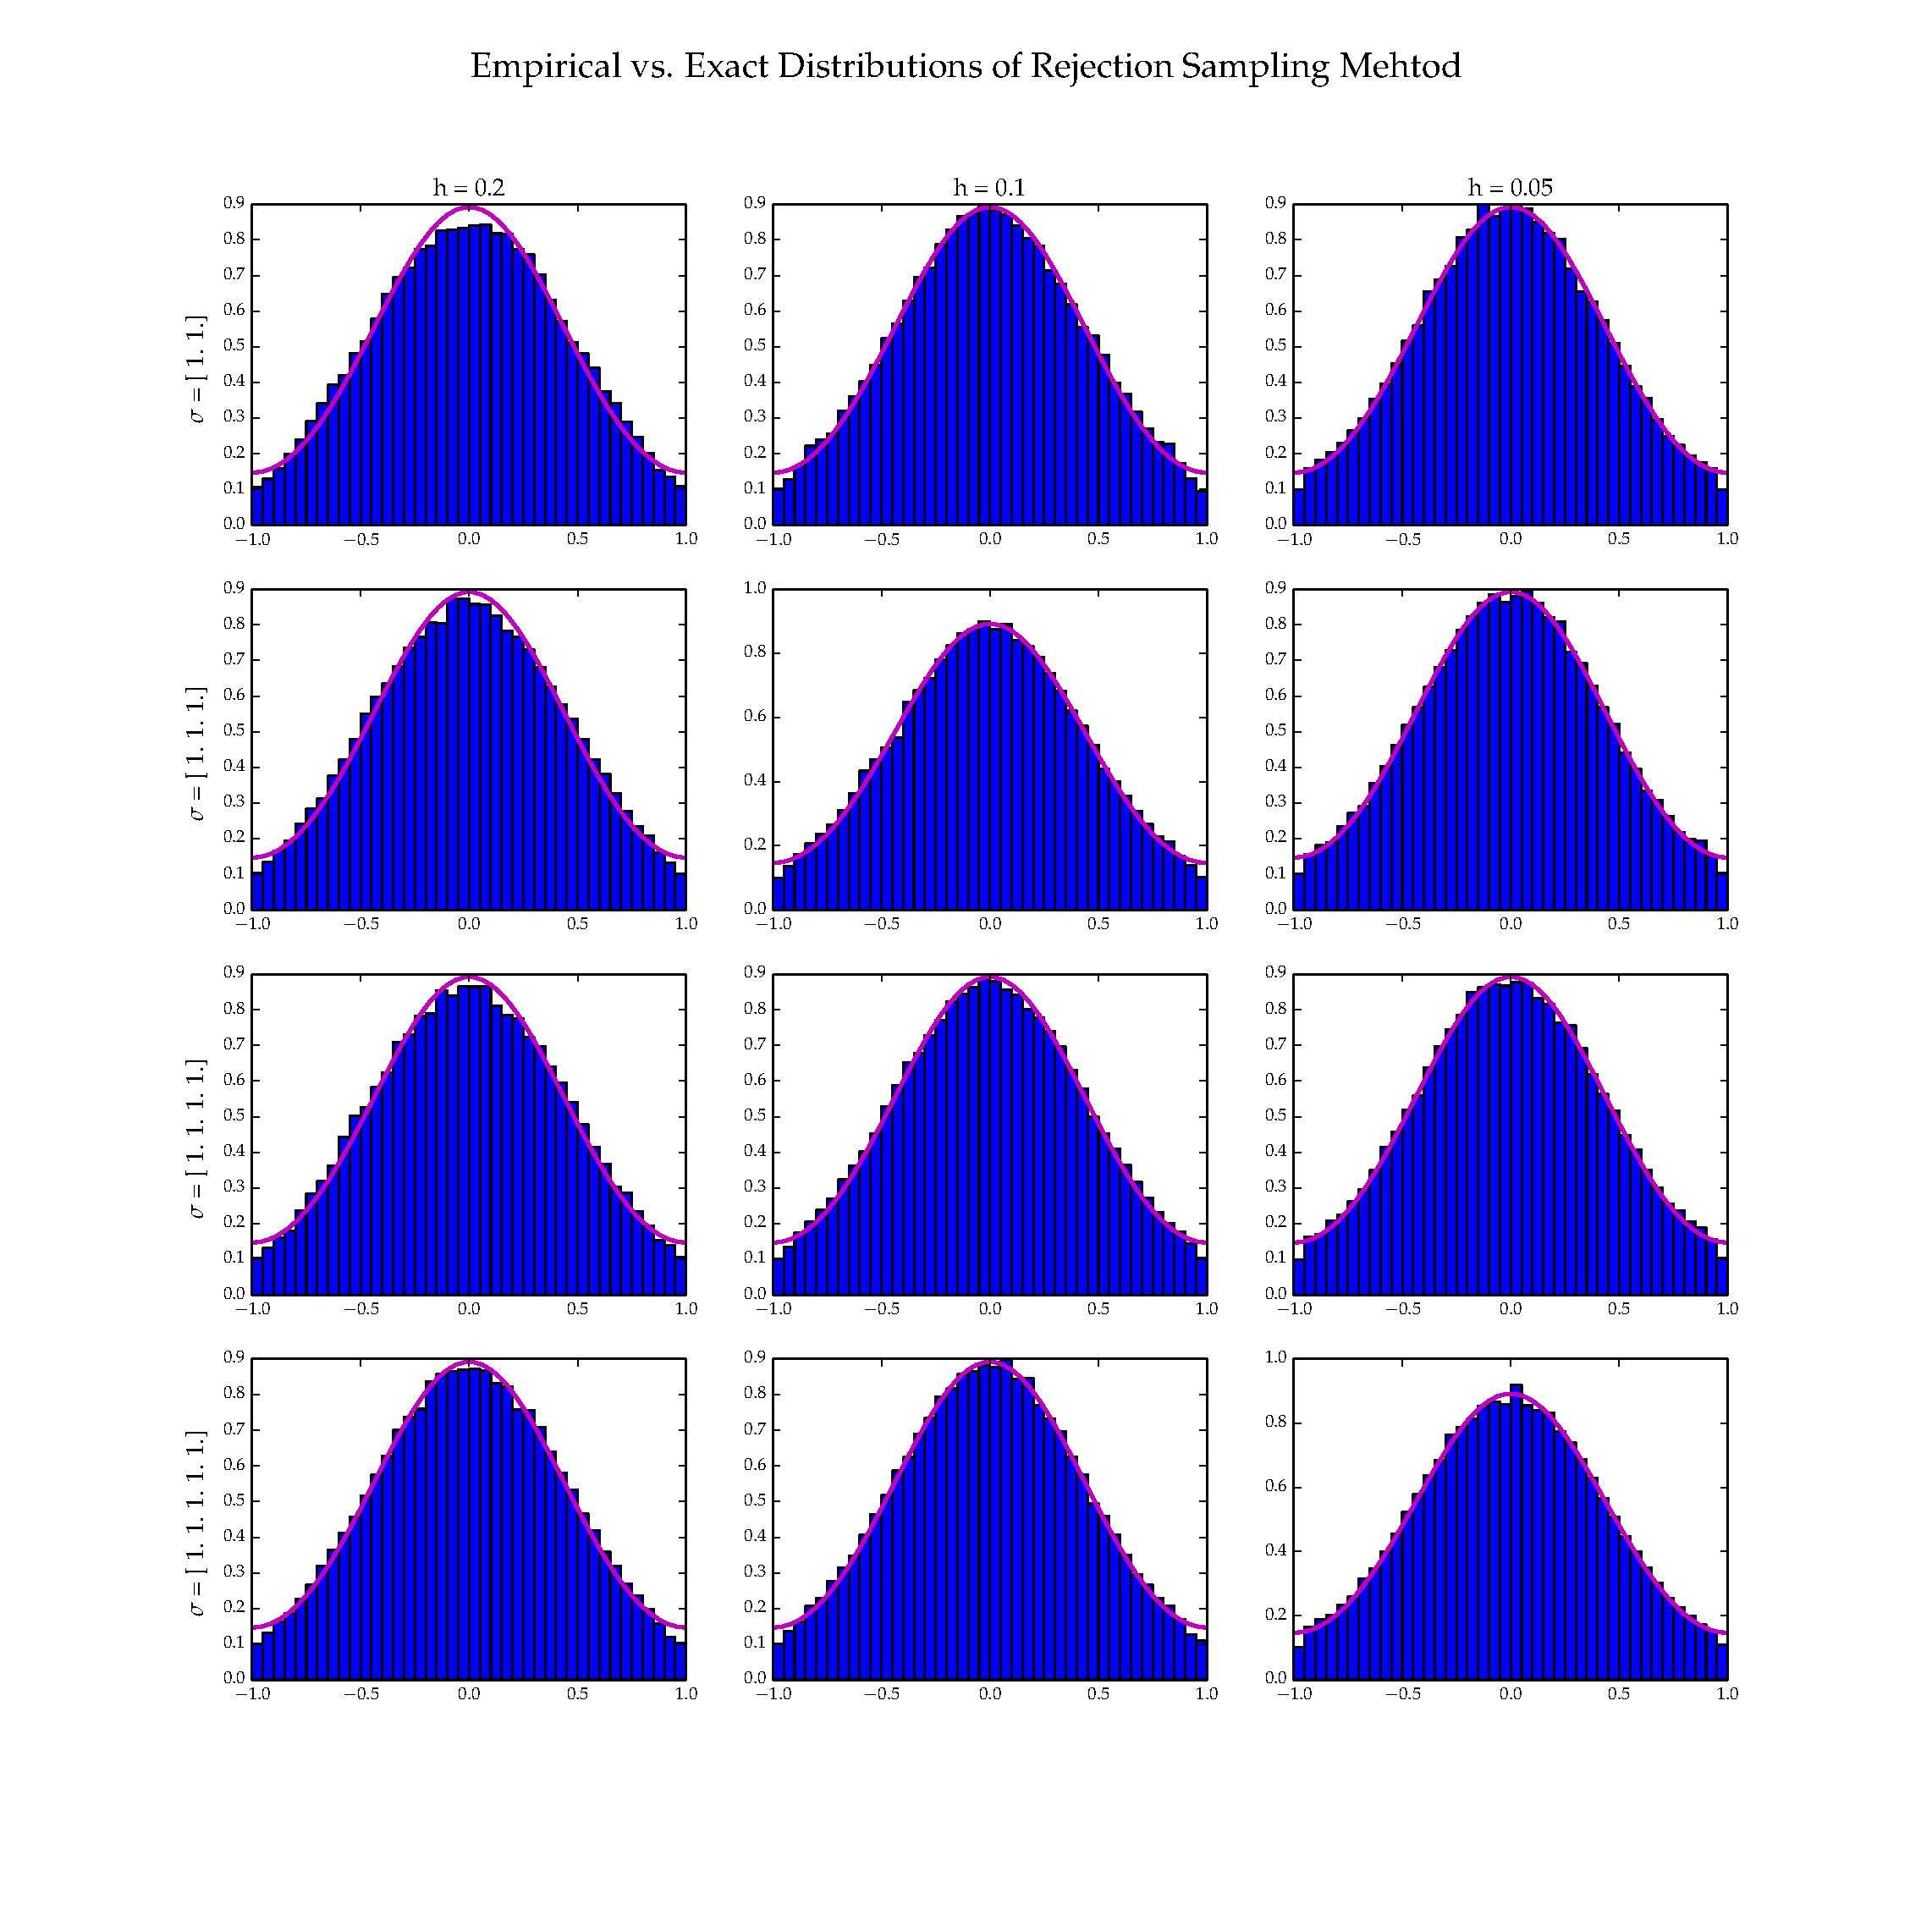
\includegraphics[scale=0.4, angle=0]{images/rejection_finite.eps}
\caption{Finite time distribution of first dimension of rejection sampled points in hyper-cubes of increasing dimension across different choices of timestep.}
\label{fig:HCFin}
\end{figure}
The results match almost perfectly with the biggest errors occurring at the boundaries. This is to be expected since the rejection method is biases the sampling slightly to points away from the boundary. 

\subsection{MRBM on Geometric Configuration Spaces}
Now, we again consider the two and three triangle linkage examples from section~\ref{ssc:MBMGCS}. Figure~\ref{fig:T2_2} depicts the same conditions (no fixed trivial degrees of freedom) as figure~\ref{fig:T2_1} previously, but with the addition of boundaries that prevent the two triangles from rotating through each other. The agreement in the two histograms is strong with the greatest differences being at the boundary as expected. 
\begin{figure}[ht]
\centering
  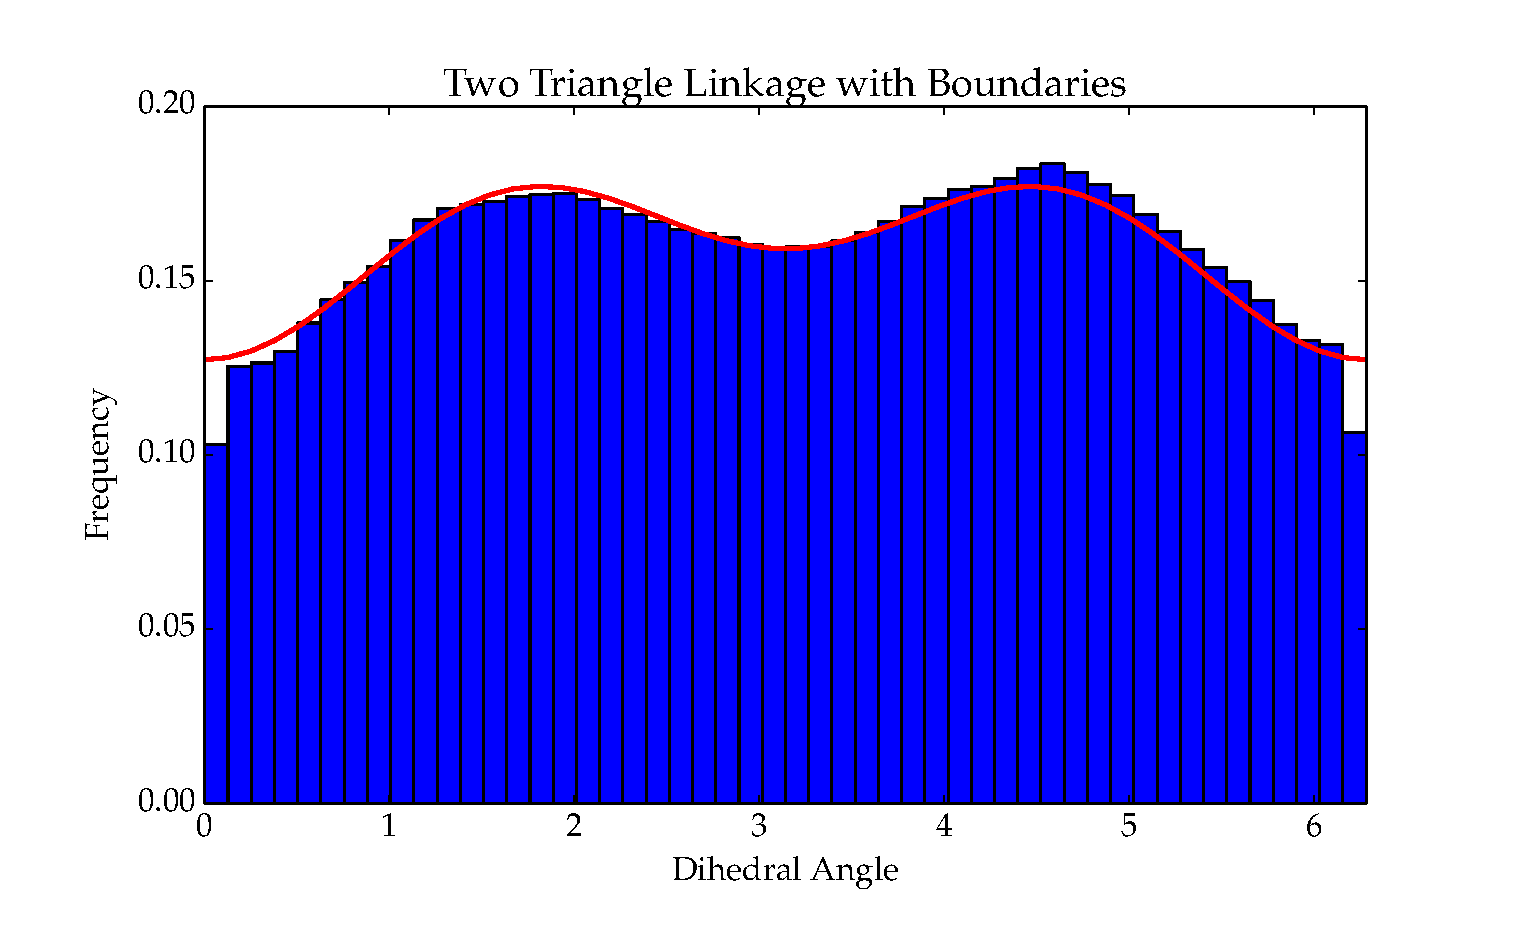
\includegraphics[scale=0.6]{images/T2_2.eps}
\caption{Sampling of two triangle linkage with boundaries.}
\label{fig:T2_2}
\end{figure}

Similarly, we consider the three triangle linkage with no fixed degrees of freedom and impose boundaries. This test is less trivial than the two triangle linkage since the exterior triangles of the linkage may interact more easily. Comparing the original in figure~\ref{fig:T3_1}, there is nice agreement except in the regions in the lower-right and upper-left corners of the plot which correspond to the aforementioned triangle intersection. Also, a noticeable layer of lower probability is seen around the periphery of the plot which reflects the boundary preventing the triangles from rotating through each other.
\begin{figure}[ht]
\centering
  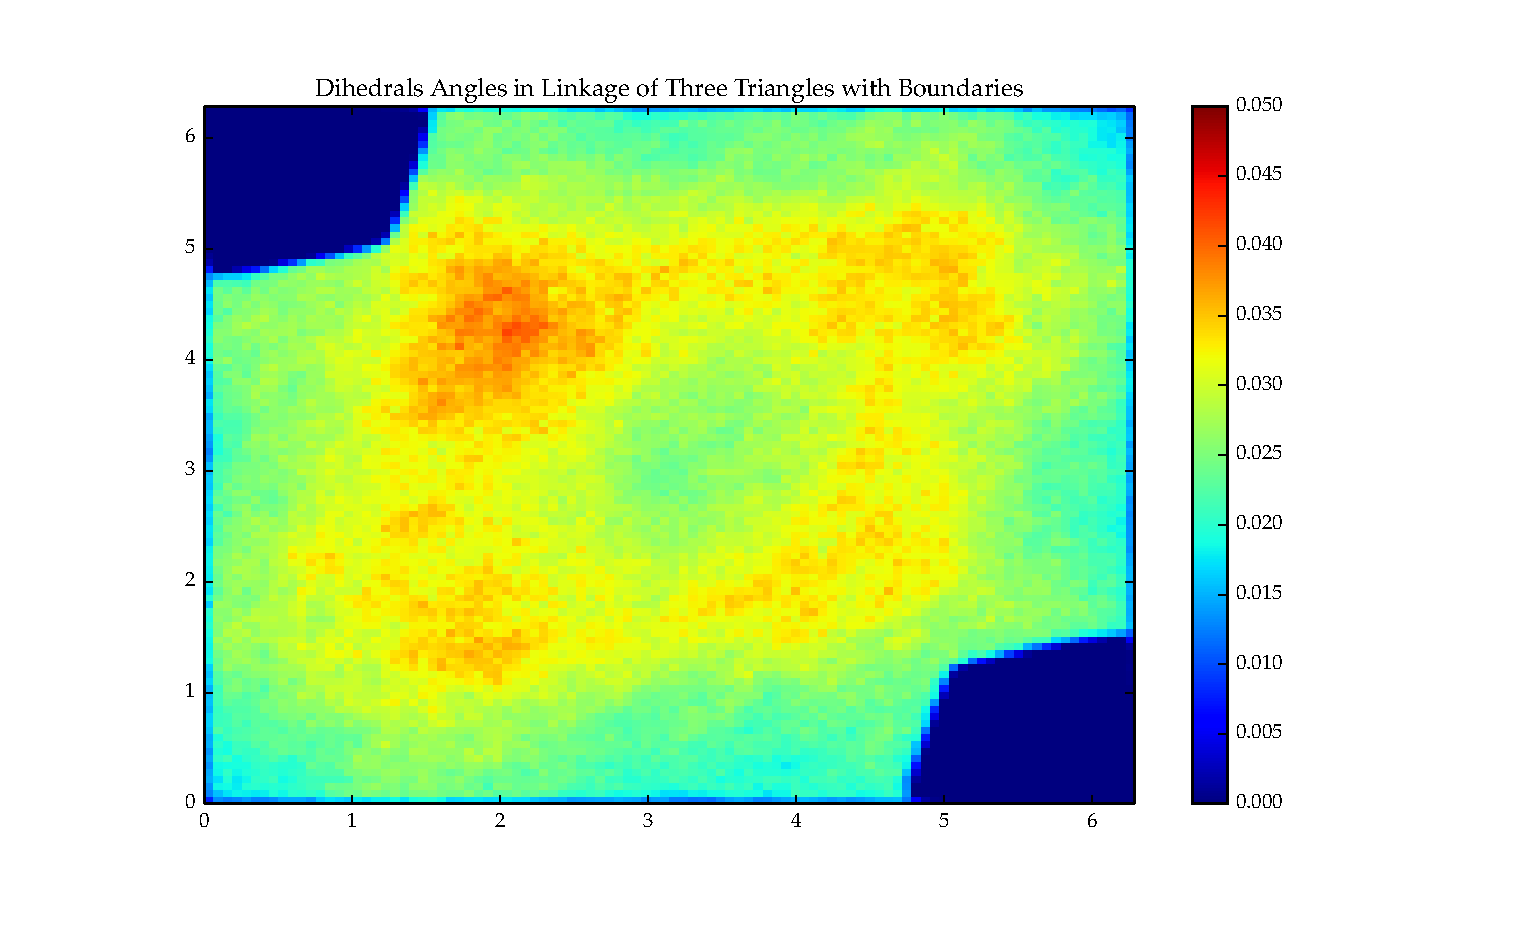
\includegraphics[scale=0.6]{images/T3_2_2D.eps}
\caption{Sampling of three triangle linkage with boundaries.}
\label{fig:T3_2}
\end{figure}


\begin{figure}[ht]
\centering
  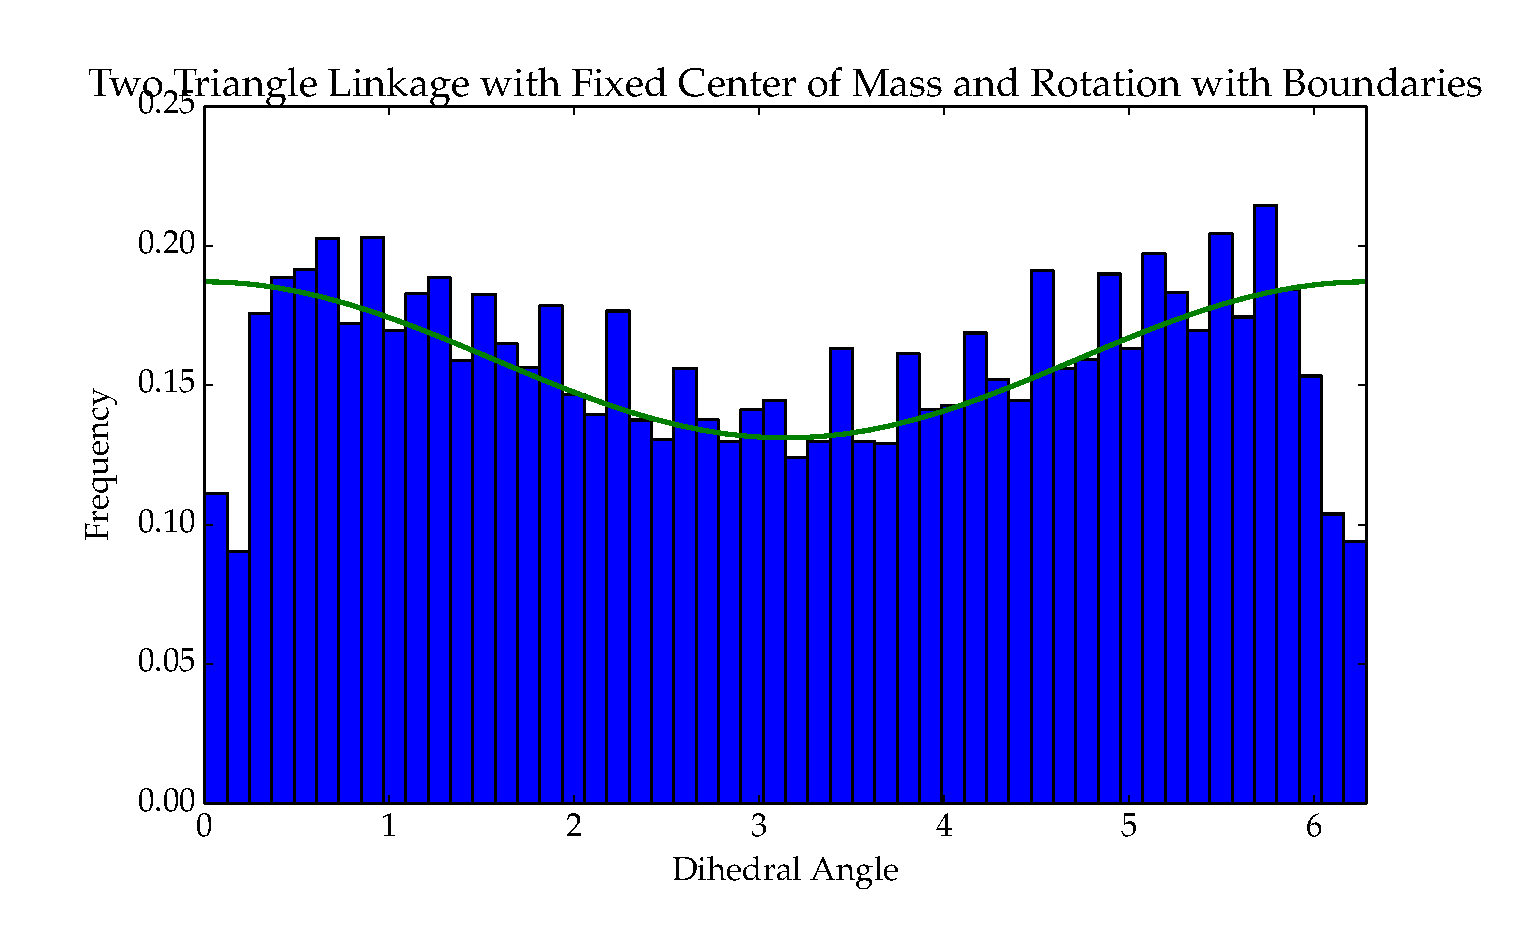
\includegraphics[scale=0.6]{images/T2_6.eps}
\caption{Sampling of two triangle linkage with boundaries and fixed center of mass and rotations.}
\label{fig:T2_6}
\end{figure}

\begin{figure}[ht]
\centering
  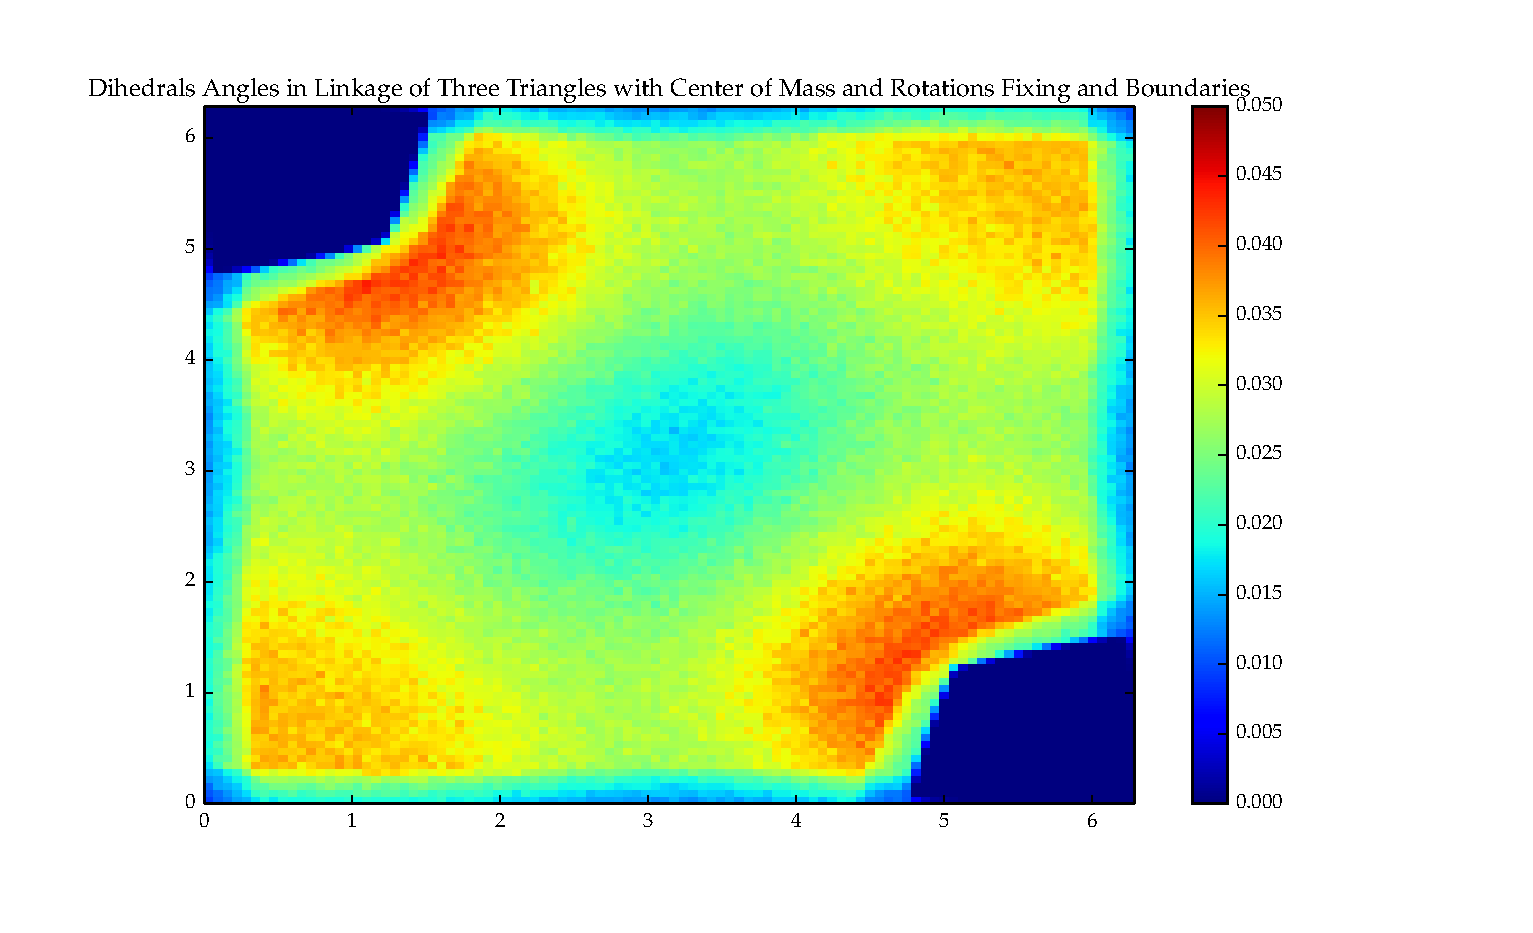
\includegraphics[scale=0.6]{images/T3_7_2D.eps}
\caption{Sampling of three triangle linkage with boundaries and fixed center of mass and rotations.}
\label{fig:T3_7}
\end{figure}


Now we compare the analogous cases in which we fixed all of the trivial degrees of freedom with and without a boundary. Figure~\ref{fig:T2_6} is the boundaried version of figure~\ref{fig:T2_5} and figure~\ref{fig:T3_7} is the boundaried version of figure~\ref{fig:T3_6}. Both cases exhibit a close comparison to their counterparts with the regions near the boundary possessing the largest deviations. 

\section{Computational Implementation}

As with our enumeration work, simulations were carried out on a desktop computer running 64-bit Ubuntu 14.04 LTS with 15.6 GiB memory and a quad-core 3.20GHz Intel processor. The module for simulating the manifold Brownian motion was implemented in Python and was able to sample at a rate on the order of $3,000,000$ samples per hour. This rate varies with use of a boundary and the dimension of the manifold and ambient spaces as well. 
